\chapterNo{Annexe A - Cahier des charges}
Ce cahier des charges a pour objectif de présenter le projet \COREL et d’en définir précisément les besoins et objectifs. Il contient un état des lieux des outils et sources, ainsi qu’une description des livrables attendus. Quelques préconisations techniques pour répondre à ces objectifs sont faites en fin de document.

\section*{Les enjeux}
Le projet \COREL fait l’objet d’un financement \CollEx Persée jusqu’au mois d’octobre 2024 et doit créer, durant cette période, un outil qui répond aux besoins des chercheurs. Cet outil devra être créé à partir d’un corpus vaste, dont les données sont issues de plusieurs sources \footnote{À ce sujet, voir la présentation du corpus.} et hétérogènes (existantes au format \XML, \csv, etc. \footnote{À ce sujet, voir l’état des lieux.}), afin de proposer aux chercheurs une architecture qui agrège les différents outils mis au service du projet, réutilisable par la communauté scientifique. 

De plus, le projet s’inscrit dans un champ disciplinaire particulier, la sinologie et l’histoire du droit. Les outils utilisés devront permettre, dans cette perspective scientifique, de montrer comment évolue le droit. 
\newpage
\section*{Contextualisation du projet}
\subsection*{Le projet \COREL}
Le projet \href{https://www-test-collex.inist.fr/projet/corel/}{\COREL} a pour but la reconstitution de la législation de la Chine impériale tardive à partir de différents corpus : des documents conservés dans les fonds du porteur de la filière IST (\cdf) et sur le travail accompli dans le cadre de programmes de recherche antérieurs (\LSC, \EPJ). Ce projet est un moyen de préserver et de valoriser ce corpus de recherche sur l’histoire juridique, en proposant une édition en ligne des textes de loi sous la dynastie Qing et un accès facilité aux documents sources via un site internet. La recherche sera également facilitée pour les chercheurs grâce à un \textit{code virtuel} \footnote{La notion de “code virtuel” renvoie à un texte de loi reconstitué artificiellement grâce aux différentes versions du code publiées entre 1644 et 1911. Une définition plus approfondie en est donnée dans les livrables du projet. } qui retracera, année après année, l’évolution du droit de 1644 à 1911. 

\subsection*{Projets précédents}
\subsubsection{Legalizing Space in China (\LSC)}
Le projet de recherche Legalizing Space in China (\LSC, financement \ANR 2011-2015) a permis d’inventorier et de collecter l’essentiel du corpus de documents juridiques chinois dont dispose le projet \COREL. Le site internet \LSC propose une version texte des sources ainsi que des documents \pdf. Il dispose également d’un glossaire et de traductions partielles des textes de lois, en anglais et en français.

\subsubsection{Emerging Procedural Justice (\EPJ)}
Le projet Emerging Procedural Justice (\EPJ, financement Arqus/European Alliance pour l’année 2020), en collaboration avec Data Futures, a permis de développer une base relationnelle d’images sur serveur \IIIF associant deux éditions du code des lois de la dynastie Qing (\dq et  l'édition de 1870) et deux compilations décrivant de façon exhaustive l’évolution des lois (\genyuan et \huidian).

\newpage
\section*{Les acteurs}
\subsection*{L'équipe}
\begin{itemize}
    \item Frédéric Constant
    \item Vincent Paillusson
    \item Luca Gabbiani
\end{itemize}

    L’équipe collabore avec le prestataire, Data Futures, ainsi qu’Huma-Num qui héberge et maintient la base de données du projet \LSC.
\subsection*{Les acteurs institutionnels}
La \href{https://www.college-de-france.fr/fr/bibliotheque-archives/bibliotheque-etudes-chinoises}{bibliothèque d’études chinoises} du \href{https://www.college-de-france.fr/fr}{Collège de France} met à la disposition du projet les documents sources sur lesquels s’appuie le projet. C’est le porteur administratif du projet. Le Centre de hautes études chinoises (anciennement Institut des hautes études chinoises) est rattaché au Collège de France et abrite la bibliothèque d'études chinoises, fondée en 1927 par Paul Pelliot et Marcel Granet. Celle-ci dispose d’une des plus importantes collections sinologiques d’Europe. Les fonds atteignent 150 000 volumes. Elle est spécialisée dans les recherches sur la sinologie classique (pré-1912) et conserve de nombreuses monographies locales anciennes (difangzhi 地方志), des collectanea (congshu 叢書, 1 400 titres) ainsi que des manuscrits rares. Elle possède aussi plusieurs éditions originales d’ouvrages utilisés dans le cadre du présent projet, dont certains exemplaires uniques au monde. La bibliothèque a reçu en mai 2021 le label \CollEx.

L’\href{https://www.efeo.fr/index.php}{École Française d’Extrême-Orient} (\EFEO) et l’Université de Nice sont chargés de l’exploitation scientifique du projet. 

L’\EFEO fondée en 1900 à Saigon, a pour mission la recherche interdisciplinaire sur les civilisations asiatiques, de l'Inde au Japon. L'\EFEO est présente, grâce à ses 18 centres de recherche, dans 12 pays d'Asie. Cette spécificité permet à ses 42 chercheurs permanents (anthropologues, archéologues, linguistes, historiens, philologues, sociologues des religions, etc.) d'être sur les terrains de leurs études, et d'animer un réseau de coopérations locales et d'échanges internationaux entre scientifiques orientalistes. L’\EFEO apporte les compétences techniques nécessaires à la réalisation du projet. 

Par l’excellence des établissements de recherche qui la composent et son potentiel d’innovation, \href{https://univ-cotedazur.fr/recherche-innovation}{Université Côte d’Azur} s’inscrit dans une politique de site ambitieuse. CNRS, INRIA, INSERM, INRAe, IRD… les instituts de Recherche nationaux constituent le socle solide d’une recherche pleinement intégrée à l’écosystème universitaire. La recherche s’exerce au travers de plus de 50 Unités Mixtes de Recherche et laboratoires. Plus de 1 200 chercheurs engagés dans des activités de Recherche fondamentale et appliquée sont impliqués dans des réseaux nationaux et internationaux. Ils sont également des acteurs majeurs dans le développement de l’innovation et le soutien de l’économie sur le territoire azuréen.

\subsection*{Prestataires}
\href{https://www.data-futures.org/}{Data Futures GmbH} est une entreprise à but non lucratif située à Leipzig et travaille sur les technologies de redistribution et de préservation des données de recherche ainsi que sur les infrastructures associées. Le partenariat Hasdai entre des institutions européennes et américaines est géré par Data Futures GmbH et est régi par un accord avec le CERN. Hasdai a étendu la technologie du dépôt Invenio du CERN aux sciences de la vie, aux sciences sociales et aux sciences humaines. Il exploite également un réseau de dépôts et d'archives InvenioRDM au nom de ses partenaires. Invenio constitue la base technique de Zenodo, le dépôt universel pour les données de la recherche, soutenu par le CERN au nom de OpenAIRE.

L’\href{https://www.huma-num.fr/quest-ce-que-l-ir-huma-num/}{IR* Huma-Num} a pour mission principale de construire, avec les communautés et à partir d’un \href{https://www.huma-num.fr/conseils-et-comites/}{pilotage scientifique}, une infrastructure numérique de niveau international (nœud français des ERIC \href{https://www.huma-num.fr/infrastructures-europeennes/#dariah}{DARIAH} et \href{https://www.huma-num.fr/infrastructures-europeennes/#clarin}{CLARIN}) pour les SHS. 

Elle structure, par l’intermédiaire de \href{https://www.huma-num.fr/les-consortiums-hn/}{consortiums} regroupant des acteurs des communautés scientifiques et d’un \href{https://www.huma-num.fr/trouver-son-relais-msh/}{réseau de points de présence dans les maisons des sciences de l’Homme (MSH)}, l’accompagnement des communautés scientifiques SHS en matière d’infrastructure numérique pour les données de la recherche. 

Elle met en œuvre une infrastructure numérique permettant aux communautés SHS de développer, de réaliser et de préserver sur le long terme les programmes de recherche – leurs données et outils- dans un contexte de science ouverte et de partage des données. 

L’ensemble de l’infrastructure s’inscrit dans le cadre des principes dits \fair (Facile à trouver, Accessible, Interopérable, Réutilisable) qui favorisent, outre l’ouverture des données, leur mise à disposition avec un triple objectif de qualité des données et des métadonnées, d’inscription dans un cycle de vie maitrisé par les scientifiques et enfin de pérennité des données sur le long terme (accès, intégrité, contextualisation de la production des données). 

Huma-Num IR* est une infrastructure de recherche « étoile », du Ministère de l’enseignement supérieur et de la recherche, mise en œuvre par le CNRS avec le Campus Condorcet et Aix-Marseille université. 

Elle est, avec son entrepôt de données NAKALA, l’un des Centres de référence de l’écosystème national Recherche Data Gouv. Engagée dans l’European Open Science Cloud, elle porte la participation de la France dans l’European Research Infrastructure Consortium (ERIC) DARIAH.
\newpage

\section*{Les objectifs}
Le projet \COREL dispose de plusieurs objectifs. Le premier est de diffuser en ligne un corpus de textes de lois de la Chine Impériale. Ce corpus sera publié sur un site internet créé pour le projet et mis à la disposition des chercheurs en droit chinois. L’objectif est de le rendre exploitable par les utilisateurs, c’est-à-dire que les textes seront consultables et recherchables. 

Cet objectif en entraîne un deuxième, qui est la reconstitution de l’évolution de la législation sous la dynastie Qing. Les sources seront regroupées sur un seul site internet, ce qui en facilitera l’accès. Grâce à ce corpus, la publication de visualisations et la génération d’un \og code virtuel\fg, c’est-à-dire un texte de loi qui reconstitue artificiellement un code légal pour une année donnée, permettra d’étudier l’évolution de la législation, année après année. 

Le troisième objectif du projet est de fournir aux porteurs du projet un site internet pérenne, qui sera modifiable, notamment pour en enrichir le contenu, en interface graphique.
\newpage
\section*{Les évolutions possibles}
L’un des objectifs du projet est de créer un site internet qui pourra évoluer avec le temps. Le projet \COREL possède en effet des perspectives d’enrichissement, notamment l’intégration de sources sur les jugements, les cas et les peines. Ces documents sont en cours de numérisation par la bibliothèque d’études chinoises du Collège de France. 

Ces documents seront directement liés au corpus : il ne s’agit pas simplement d’ajouter de nouveaux documents, mais de permettre aux chercheurs de mettre ces documents en relation. Certains cas ou jugements donnent naissance à des lois et il serait intéressant de pouvoir lier ces textes aux lois. 

De plus, un dépôt des images résultant de la numérisation du code est envisagé sur \href{https://www.nakala.fr/about}{Nakala}. 

\newpage
\section*{Les contraintes}
Le projet \COREL possède un financement limité dans le temps, jusqu’au mois d’octobre 2024 et devra donc être réalisé dans le temps imparti. De plus, les données mises à notre disposition sont hétérogènes : données \XML, exports de Freizo (\csv, \JSON), etc. \footnote{Voir l’état des lieux. }

Le projet s’appuie sur des projets précédents et cherche donc à s’inscrire dans la continuité de ceux-ci. Pour cela, la reproduction partielle du site Legalizing Space in China est envisagée. \footnote{Voir les maquettes et la partie édition en ligne.}

Ce projet d’humanités numériques doit de plus garantir la maintenabilité des livrables dans le temps, en utilisant des outils open-source et bien documentés. Ces outils devront être accessibles en interface graphique aux chercheurs qui n’ont pas de compétences techniques et devront être choisis pour leur flexibilité, afin de laisser ouverte la possibilité d’une évolution du projet dans le temps. 

Le projet ne souhaite pas créer un site web via un développement customisé et souhaite utiliser un outil accessible et exploitable librement, avec une documentation disponible en ligne, et une communauté d’utilisateurs bien développée. Cet outil devra permettre de diffuser les textes de lois en ligne, personnaliser l’affichage et pouvoir ajouter des pages au site internet avec un système de gestion de contenu, sans nécessité de coder. L’ajout, la suppression ou la modification des pages doit être accessible en interface graphique. Cet outil doit aussi intégrer un système de gestion de base de données \XML pour pouvoir gérer la base de données du projet et l’enrichir. L’outil utilisé pour le projet doit être open-source et ne doit pas dépendre d’un tiers, que ce soit pour le développement ou la maintenance (qu’elle soit corrective ou évolutive).

\newpage
\section*{Présentation du corpus}
La bureaucratie chinoise de l’époque impériale rendait la justice en application de codes promulgués en général en début de dynastie et régulièrement mis à jour. La première édition du code publiée sous la dynastie Qing date de 1646 et contient plusieurs centaines d’articles ; la dernière, promulguée en 1870, en regroupe environ 2000. Si l’on ajoute les dispositions entre temps abrogées ou modifiées, la législation Qing a compris plusieurs milliers d’articles. Par ailleurs, le droit chinois évoluait lorsque des édits élevaient au rang de loi des décisions rendues dans des affaires importantes ou à la suite de mémoires proposant une modification du droit. La relation entre les lois et les jugements n’était pas univoque et il existait une dynamique complexe entre les deux sources.

Une révision du code est faite environ tous les 10 ans, il existe 23 éditions successives des codes chinois mais seulement une partie a été conservée. Notre corpus est constitué de quatre éditions sur la période 1644-1911.
Un premier texte de loi a été publié en 1646. Le deuxième est paru en 1740. Ce code fixe les \lu, les lois principales, de manière définitive. Elles ne sont plus modifiées ensuite. Ces codes comprennent aussi les \li, des lois secondaires qui font partie du droit vivant. Les \lu se réduisent au fur et à mesure, tandis que les \li augmentent. Les codes sont divisés en 7 chapitres, dans lesquels se trouvent les sections, les lois principales, puis les lois secondaires. La division en chapitres correspond aux différents ministères.

Le \textit{Da Qing lüli genyuan 大清律例根源} présente les lois additionnelles organisées de manière chronologique, donc dans l’ordre de modification du code. 
Le \textit{Huidian shili 會典事例} est un texte de 1899 qui compile l’ensemble des lois en vigueur ainsi que les textes abrogés. Il organise les lois en classant les \li selon la loi principale à laquelle elles sont rattachées.

Le \textit{Duli cunyi 讀例存疑} est un texte de 1906, qui compile les lois en vigueur sous la dynastie Qing avec des explications historiques. Il a été établi par Xue Yuncheng pour aider à la révision du code des Qing.

Ces quatre sources permettent de reconstituer la législation chinoise entre 1644 et 1911, mais cela nécessite de croiser les informations. Certaines lois sont présentes dans plusieurs ouvrages, tandis que d’autres n’ont été retranscrites que dans un seul. Il est donc nécessaire de croiser les sources. 

\newpage
\section*{L'état des lieux}
\subsection*{Les documents \XML}
\subsubsection{L’encodage XML}

Les documents sources ont été océrisés puis encodés en \XML, selon un schéma propre au site internet \LSC. La structure des textes de lois chinois (chapitres, sections, lois principales et lois secondaires) est conservée dans le balisage. 

Les documents sont conçus sur un modèle d’encodage trilingue. Chaque balise est donc répétée avec un attribut de langue différent (chinois, anglais ou français), cependant la traduction n’est pas systématique, laissant certaines balises vides. 

De nombreuses pièces liminaires (par exemple \texttt{<description>}, \texttt{<edition>}...) sont présentes pour documenter le projet d’édition \LSC ou présentent du contenu additionnel aux codes légaux. Ces éléments n’ont pas été repris dans le projet \COREL, à l’exception des tableaux synoptiques qui apparaissent au début du code de 1740. Ils donnent une vue d’ensemble sur des catégories transversales, par exemple le montant à verser pour racheter une peine. 

L’encodage \XML est lié à l’affichage du site internet \LSC. Certaines balises \HTML sont utilisées dans l’encodage \XML, par exemple des balises \texttt{<i>}, qui affichent le texte en italique. Les balises \texttt{<inf>}, créées pour le projet \LSC, permettent d’afficher le texte en caractères plus petits, en bleu. 

\subsubsection{La transformation en XML-TEI}
\textbf{Pourquoi la TEI ? }

La \TEI (\href{https://tei-c.org/}{Text Encoding Initiative}) propose un standard d'encodage préconisé pour l'édition scientifique. Elle est largement utilisée dans le domaine de la recherche et offre une documentation en ligne complète. La \TEI permet d'encoder les textes de manière sémantique en distinguant la forme (l'affichage) du fond (le contenu intellectuel). L'encodage en \XML-\TEI assure également l'interopérabilité des données, favorisant l'échange et la collaboration entre les projets de recherche.
Les documents \XML encodés pour le site \LSC ont été transformés via une feuille de style \XSL en \XML-\TEI. Cette transformation a été motivée par deux objectifs : utiliser un balisage sémantique, contrairement au balisage \XML original qui était lié à l’affichage du site internet, pour structurer les documents, et se conformer à un langage universel, préconisé pour l’édition scientifique. Son utilisation s’insère dans une culture métier et scientifique déjà fortement impactée par son usage. De plus, le choix de balises du schéma \LSC devenait trop restreint pour un balisage sémantique (une liste de balises restreinte était prise en compte sur le site internet). Le passage à la \TEI permet de choisir des balises plus adaptées à chaque élément des sources.

Cette transformation a permis d’établir un \href{https://sharedocs.huma-num.fr/wl/?id=yHHcUPKWyusazIZqWVLgtbZI7J65OaLA&path=TEI%282%29&mode=grid}{jeu de données de référence} : la conversion en \TEI reprend toutes les informations nécessaires au projet \COREL présents dans les documents \XML à l’heure actuelle. Ce jeu de données est encore partiel : il manque certaines données dans les documents \XML qui devront être récupérées afin de les intégrer à l’encodage \TEI.
\bigskip
\textbf{Choix d’encodage}
Les documents \XML ayant été encodés pour le projet précédent (\LSC), toutes les données ne sont pas pertinentes pour le projet \COREL. Seuls les éléments structurants des documents ont été conservés et transformés en balises \TEI. C’est le cas des chapitres (\textit{bu}), sections (\textit{men}), lois principales (\textit{lü}) et lois secondaires (\textit{li}). 

Le passage à la \TEI a également permis de sémantiser certaines balises \XML qui étaient liées à l’affichage sur le site internet \LSC, notamment les balises \texttt{<inf>} qui sont des commentaires officiels du code. Un \href{https://sharedocs.huma-num.fr/wl/?id=yHHcUPKWyusazIZqWVLgtbZI7J65OaLA&path=ODD&mode=grid}{guide d’encodage} a été rédigé pour ces documents. 

Les documents \TEI sont constitués d’un \texttt{<teiHeader>} qui contient les métadonnées relatives aux documents sources et à l’édition en ligne. 

\noindent 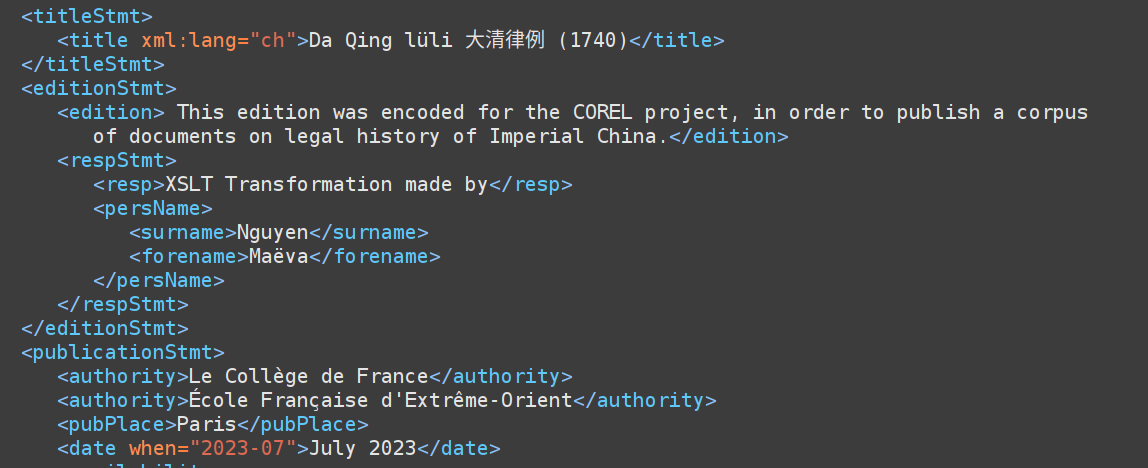
\includegraphics[width=\textwidth]{images/annexe1.png}

Chaque document est contenu dans une balise \texttt{<text>} avec deux attributs : un attribut de langue (le chinois) et un identifiant unique qui permet d’identifier le code légal. 

\noindent 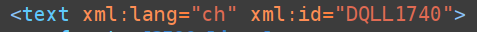
\includegraphics[width=\textwidth]{images/annexe2.png}

Les chapitres, sections et lois sont contenues dans des balises \texttt{<div> }imbriquées. Ces balises ont obligatoirement un attribut \texttt{@type} et une numérotation. Elles sont immédiatement suivies d’une balise autofermante \texttt{<pb/>}.

\noindent 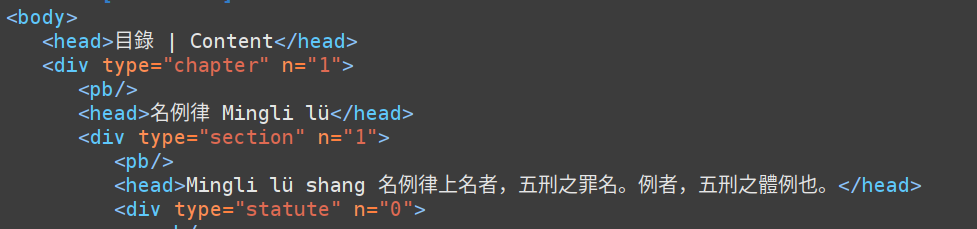
\includegraphics[width=\textwidth]{images/annexe3.png}

Les commentaires contenus dans le code légal sont marqués par une balise \texttt{<note>} dont l’attribut \texttt{@type} est \og official \fg. 

\noindent 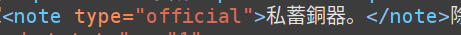
\includegraphics[width=\textwidth]{images/annexe4.png}

Le \huidian contient également des listes qui sont balisées comme suit. Chaque élément de la liste (\texttt{<item>}) contient une date et un ou plusieurs paragraphes. 

\noindent 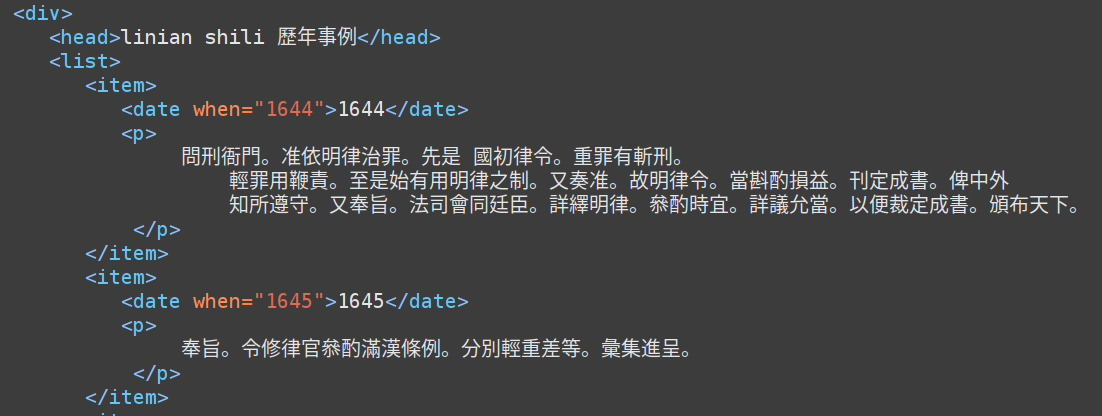
\includegraphics[width=\textwidth]{images/annexe5.png}

Les entités nommées au sein du texte ont été marquées par des balises \texttt{<persName>} pour les noms de personnes, \texttt{<placeName>} pour les noms de lieux et \texttt{<bibl>} pour les références bibliographiques. 

\subsection*{Les métadonnées \IIIF}
\subsubsection{Serveur \IIIF et annotations}

La numérisation des codes légaux a été mise en ligne via la plateforme Freizo, sur un serveur \IIIF. \IIIF (International Image Interoperability Framework) est un protocole qui permet la diffusion et l’échange d’images en haute définition sur le web. La plateforme Freizo donne accès à ces images via le visualiseur Mirador, qui offre la possibilité d’annoter les images et de les segmenter. Les annotations se font sur l’interface web dédiée et sont accessibles et modifiables en interface graphique, ainsi que via des fichiers \JSON. Cette méthode d’annotation permet aux chercheurs de relier de façon précise les métadonnées à des segments de texte. Cette partie du travail a été réalisée par Data Futures \footnote{Pour Data Futures, voir les acteurs, section ‘prestataire’.} lors du projet \EPJ \footnote{Concernant le projet EPJ, voir la contextualisation du projet.}. Les annotations permettent de déterminer le commencement d’un chapitre, une section ou une loi sur la numérisation. 

Les annotations contiennent les informations suivantes, dans cet ordre : 
\begin{itemize}
    \item   Type : le type du passage segmenté (chapitre, section, lü, tiaoli)
    \item Title (zh) : le titre en caractères chinois
    \item Title (zh-Latn) : le titre en alphabet romain
    \item Substatute : le numéro du tiaoli correspondant
    \item Related (h) : le numéro de la loi dans le Huidian Shili
    \item  Related (d) : Dulicunyi (code de 1871)
    \item  Related (c) : Code de 1740
    \item  Related (g) : le numéro de la loi dans le Genyuan
    \item Ghost : Lorsqu’une version postérieure de la loi est mentionnée dans le commentaire, sans que le texte n’apparaisse. 
    \item Date : la date de début de la loi
\end{itemize}

\subsubsection{Les métadonnées}
Les \href{https://duli-cunyi.freizo.org/browse.cgi}{métadonnées} des images \IIIF sont accessibles via Freizo. Elles contiennent le numéro d’asset (un identifiant unique attribué à chaque fichier), le titre du fichier, le titre du code (pour l’exemple ci-dessous : \textit{Huidian}), et des métadonnées (titre, auteur, producteur, date de création, etc.). Un lien hypertexte permet d’accéder au fichier sous format \PDF. 

\noindent 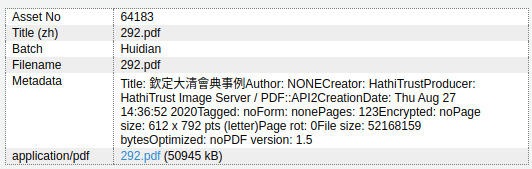
\includegraphics[width=\textwidth]{images/annexe6.png}

\subsection*{Les liens entre les lois}
Sur Freizo des liens entre les lois des différents codes ont été établis. Certaines lois sont présentes dans plusieurs codes, tandis que d’autres ne se retrouvent que dans un seul code. \footnote{À ce sujet, voir la présentation du corpus.} Il existe deux types de liens entre les lois.

\subsubsection{Des liens d'association}
Le premier lien indique les correspondances entre les lois des différents codes. Ce lien est établi à partir du \genyuan et est retranscrit ainsi : \og related duli-cunyi 1 \fg. Cela permet de donner le titre du code et le numéro de la loi correspondant à celle du \genyuan. Il contient également un lien hypertexte qui renvoie à la numérisation, via le visualiseur Mirador. 

\noindent 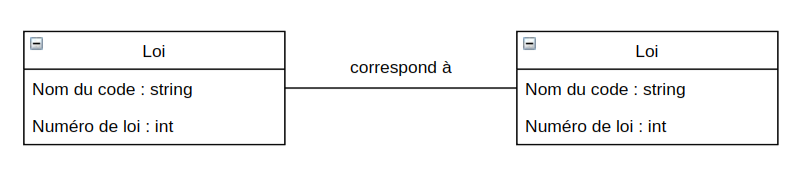
\includegraphics[width=\textwidth]{images/image4.png}

\subsubsection{Des liens d'association dirigée}
Le deuxième type de lien renvoie à des liens de filiation ou d'évolution entre les textes de loi au cours de la période étudiée. Ces relations sont qualifiées de \og \textit{in} \fg ou \og \textit{out} \fg comme ceci : 
 \og genyuan 1-35,o \fg. Le \textit{o} signale une relation \textit{out}, c’est-à-dire que la loi dont on parle prend fin et donne naissance à la loi 1-35 référencée dans le \genyuan. \og genyuan 1-10,i \fg signale une relation \textit{in}, c’est-à-dire que la loi dont il est question est issue de la loi 1-10 recensée dans le \genyuan. 

 \noindent 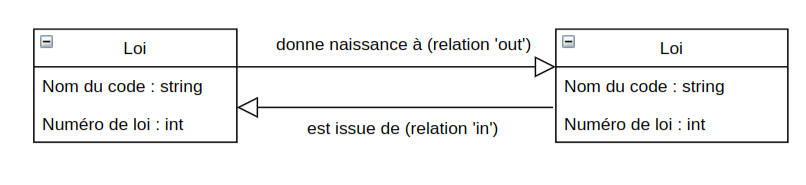
\includegraphics[width=\textwidth]{images/image5.png}

 Ces données ont été exportées au format \csv et/ou \tsv. Un \href{https://sharedocs.huma-num.fr/wl/?id=yHHcUPKWyusazIZqWVLgtbZI7J65OaLA&path=Export_Freizo%2Fgenyuan%20test.xlsx&mode=grid}{premier tableau} contient : 
 \begin{itemize}
     \item le numéro d’asset : un identifiant unique attribué à chaque fichier
    \item  le numéro de page
    \item  une URL qu’il est possible de reconstituer en faisant précéder celle-ci : 
    
    \small \texttt{https://www.google.com/urlq=https://dulicunyi.freizo.org/mirador/ \\book.cgicatno\%3D28941\%26canvas\%D\&sa=D\&source=docs\&ust=1685005327813312\&usg= \\ AOvVaw2BH\_xnL-xkCyTTj4QaCgEy} 
    et en modifiant le numéro catno pour qu’il corresponde au document recherché.
    \item le level : le type de workflow de Freizo
    \item  le titre en chinois
    \item  l’identifiant ‘related’ qui permet d’établir le lien entre les lois
    \item  la date de début de la loi
    \item  l’identifiant qui permet les relations avec les autres textes de loi
 \end{itemize}

Le \href{https://sharedocs.huma-num.fr/wl/?id=yHHcUPKWyusazIZqWVLgtbZI7J65OaLA&path=Export_Freizo%2Fdc-anno-dump-2002-04-14-v2.xls&mode=grid}{second} contient les informations suivantes : 
\begin{itemize}
    \item ressource : une URL
    \item annotatedBy : le nom de l’auteur de l’annotation
    \item  date : la date de début de la loi
    \item  subtype : le type de loi (statute, substatute)
    \item  huidian : le lien vers le Huidian
    \item  dulicunyi : le lien vers le Duli cunyi
    \item  genyuan : le lien vers le Genyuan
    \item  code\_1740 : le lien vers le code de 1740
    \item  title\_zh : le titre en chinois
    \item  number : l’identifiant Freizo
    \item  origin : des informations sur l’origine de la loi
    \item modifications : type de modification apportée à la loi (abrogation, fusion..)
    \item  correspondance : Correspondance avec un autre corpus
    \item related : le numéro de la loi décrite dans le workflow Mirador 2. Les commentaires peuvent être situés avant ou après la loi, il est donc nécessaire de rattacher le commentaire à un segment de texte.
    \item  centraladmin: décision prise par l’administration centrale. Indique également quelle administration est intervenue.
    \item  officialname : le nom du fonctionnaire 
    \item officialfunction : la fonction occupée par le fonctionnaire
    \item  province : le nom de la province
    \item  localadmin : Administration locale ayant rendu le jugement (information de type géographique)
    \item  partyname : Nom des personnes parties à une affaire
    \item original : référence du document original
\end{itemize}
\newpage

\section*{Les livrables du projet}
Le projet \COREL a pour objectif de produire deux livrables pour octobre 2024 : un site internet qui contient l’édition en ligne des textes ainsi que la recomposition de la législation pour une année donnée. Le projet souhaite produire un \POC (Proof of concept) sur un échantillon de lois afin de démontrer la faisabilité du code virtuel. Ce \POC est l’engagement minimal pris auprès de \CollEx Persée pour le financement du projet. Il consiste à générer le code virtuel sur une petite quantité de données (3 lois représentatives).

Tous les livrables du projet, ainsi que les données produites, seront publiés sous la licence \href{https://www.etalab.gouv.fr/licence-ouverte-open-licence/}{Etalab}.

\subsection*{Le site internet}
\subsubsection{Le public cible}
Le premier public visé est la communauté des sinologues, et plus particulièrement les chercheurs qui étudient l’histoire du droit chinois ou utilisent les sources juridiques pour mener des études en histoire sociale, économique ou politique de la Chine, champs d’investigations pour lesquels ces sources sont devenues un matériau essentiel. Le projet vise à mettre à la disposition de ces chercheurs un outil permettant de consulter de nombreux documents pour le moment difficilement accessibles, et d’explorer aisément des données qui n’ont pas encore fait l’objet d’un inventaire et d’une indexation systématiques. 

\subsubsection{Les besoins utilisateurs}
Le premier besoin des utilisateurs est d’avoir accès à une plateforme qui regroupe les différentes sources du droit chinois. En effet, ces sources sont partielles et se complètent les unes les autres, c’est pourquoi proposer une édition en ligne de ces textes est nécessaire pour les chercheurs. L’édition en ligne devra donc contenir les textes de lois, mais aussi des commentaires non-officiels. 

Le projet vise également à agréger ces sources afin de reconstituer la législation de la Chine impériale année après année. Cela permettrait aux utilisateurs d’avoir un accès direct et immédiat à la reconstitution de la législation de la Chine impériale entre 1644 et 1911. Le site internet doit donc être en mesure d’afficher toutes les lois en vigueur pour une année donnée. 

Les chercheurs qui s'intéressent à l’évolution du droit chinois ont également besoin de pouvoir constater l’évolution du droit sous la dynastie Qing. 

\subsubsection{Les besoins administrateurs}

Le site internet devra être entièrement accessible en interface graphique, y compris pour ses administrateurs, afin de pouvoir ajouter des documents et enrichir le site internet après son déploiement en ligne. Pour cela, le site devra proposer un back-office simple d’utilisation, qui permette de se connecter en tant qu’administrateur et de déposer de nouveaux documents, en \textit{drag and drop} ou en parcourant les fichiers de l’ordinateur. 

Les porteurs du projet ont également besoin d’un site qui soit \textbf{autonome}, c’est-à-dire qu’il doit être le moins possible contraint par un tiers. Le site doit être modifiable dans la durée par les administrateurs, sans validation préalable des documents déposés (les créateurs, propriétaires, hébergeurs, etc. du site internet ne peuvent pas refuser la modification du site par un administrateur). Ce besoin est primordial afin de se défaire de la contrainte que représente actuellement le site \LSC, qui ne peut pas être modifié sans la supervision du propriétaire.

\subsubsection{L'aspect du site web}
La description du site internet ainsi que les maquettes ont été réalisées à partir d’exemples de sites \tp, en prenant en compte les besoins utilisateurs et administrateurs. 

Le site web doit contenir une page d’accueil, une page dédiée au corpus, plusieurs pages pour consulter un à un les documents, une page qui affiche le code virtuel, une page de connexion et une page pour administrer le site en interface graphique (télécharger, supprimer, modifier des documents et ajouter de nouvelles pages au site). \footnote{Pour les maquettes du site internet, voir les annexes. }

\bigskip
\textbf{La page d’accueil}

La page d’accueil contient une barre de navigation, qui reste la même pour toutes les pages. La barre de navigation donne accès à la page d’accueil, le corpus, le code virtuel, un à propos, une barre de recherche simple et à l’onglet de connexion. L’onglet \og about \fg est déroulant et affiche l’accès à : des renseignements sur le projet, l’équipe, les mentions légales et le contact. L’onglet \og corpus \fg est également déroulant et donne accès à la liste des documents directement pour faciliter la circulation d’un texte à un autre.

La page contient également le titre du site et sa présentation. Des images avec des liens hypertexte donnent accès au corpus, au code virtuel, et à la présentation du projet. 

Le \textit{footer} du site est le même pour toutes les pages et contient les logos des différentes institutions du projet, les mentions légales, le plan du site et la page de contact. 

\bigskip
\textbf{Le corpus}

Une page affiche la liste de tous les documents disponibles sur le site internet, avec une présentation générale du corpus. La liste des documents contient un aperçu du fac similé, le titre et les métadonnées de chaque document. Ces items sont cliquables et donnent accès à l’édition en ligne de chaque document.

\bigskip
\textbf{L’édition en ligne des documents}

L’édition en ligne propose plusieurs types d’affichage différents. Le premier est un affichage simple, du texte entier et continu. Il est donc possible d’accéder à un code légal en entier sur la même page. La table des matières est navigable et cliquable. Grâce à des ancres, il est possible de naviguer dans le document. 

Le deuxième affichage propose le texte paginé. Comme \LSC, il affiche le texte en plusieurs pages et sépare les chapitres, sections, \lu et \li. En regard du texte, le visualiseur \IIIF propose le code numérisé. Le visualiseur montre la page du texte correspondant au début du chapitre, de la section ou de la loi.

Il est aussi possible d’accéder uniquement au texte paginé, sans visualiseur \IIIF. 

L’affichage du texte paginé permet aussi de choisir différents modes d’affichage. Un affichage \textit{named entities} propose de mettre en avant les entités nommées balisées dans le texte, par exemple en gras. 

Le mode \textit{metadata} permet d’afficher à côté d’une loi ses métadonnées. Ces métadonnées sont stockées dans les commentaires de type \textit{metadata}.

Le mode \textit{commentaries} permet d’afficher les commentaires en plus du texte, à la suite. Ce mode d’affichage n’inclut pas les commentaires de métadonnées des lois, qui sont à afficher dans un mode différent. 

Pour chaque affichage différent, un accès à la table des matières du document devra être disponible via un onglet flottant et indiquer clairement où l’utilisateur se situe dans l’arborescence du document (avec une fonction \textit{hover} par exemple). Cette table des matières sera cliquable pour faciliter la navigation dans le texte. 

Les métadonnées générales devront également être accessibles via un onglet flottant. 

Les titres des lois devront être cliquables afin d’accéder à la page des visualisations.

\bigskip
\textbf{Le code virtuel}

En entrée, la page du code virtuel propose un paragraphe d’explications (qu’est-ce que ce code virtuel et comment l’utiliser ?). Une barre de saisie permet à l’utilisateur de saisir une date entre 1644 et 1911. 

En sortie, le code virtuel affiche toutes les lois dont les bornes chronologiques comprennent la date donnée en entrée. L’affichage est continu, avec une table des matières cliquable qui permet de se déplacer dans le code. Une fonction d’export au format \pdf est disponible pour télécharger le résultat du code généré. \footnote{Pour en savoir plus sur le code virtuel, voir la section suivante, \og recomposition du code virtuel \fg.}

\newpage
\textbf{Une page de connexion}

La page de connexion offre un formulaire avec un nom d’utilisateur et un mot de passe. Elle permet aux administrateurs du site de se connecter et d’accéder au back-office. 

\bigskip
\textbf{Une page d'ajout de nouveaux documents}

Cette page n’est accessible qu’aux administrateurs une fois connectés. Elle propose d’ajouter de nouveaux documents en \textit{drag and drop} ou en parcourant les fichiers de l’ordinateur. 

Lorsque l’utilisateur est connecté, la barre de navigation affiche un nouvel onglet qui permet d’accéder à la page d’ajout. Pour que le document s’affiche correctement sans modifications des paramètres d’affichage, il doit respecter le schéma d’encodage choisi pour les documents.

\noindent 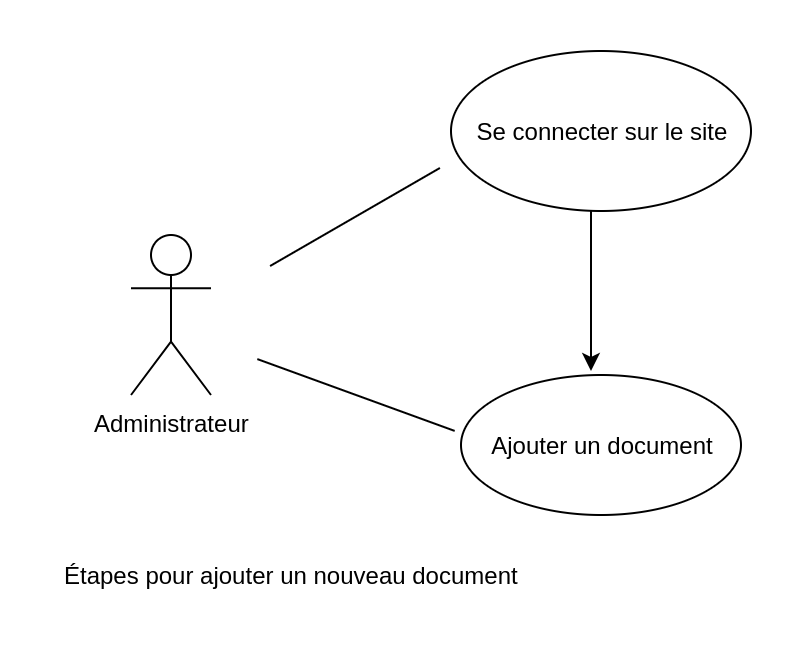
\includegraphics[width=\textwidth]{images/annexe7.png}

Si le site web est réalisé avec \tp, la suppression et la modification de documents déjà mis en ligne se fait via l’interface eXide. L’ajout de nouvelles pages au site internet est possible en encodant les pages souhaitées en \TEI ou en Markdown, ou bien en téléchargeant sur \tp un document .docx. \footnote{Cette fonctionnalité de \tp est encore en cours de développement, mais fonctionne très bien pour éditer des pages simples. Le formatage direct est conservé en grande partie (titre, caractères en gras, etc.) et permet aussi d’intégrer des images. Il y a ensuite la possibilité de personnaliser davantage cet affichage avec l’\ODD de \tp, comme pour l’édition en ligne.}

\bigskip
\textbf{Une page dédiée aux visualisations}

Le site devra proposer des visualisations de ces évolutions, et retracer la généalogie des lois à partir des liens entre les lois. \footnote{À ce propos, voir la modélisation des liens entre les lois.}  La visualisation devra être accessible via l’édition en ligne, en cliquant sur la loi dont on souhaite voir apparaître la généalogie. Pour réaliser ces visualisations, les liens entre les données sur la généalogie des lois sont disponibles dans les fichiers \JSON. 

Les schémas ci-dessous présentent des modélisations simplifiées et non exhaustives de la généalogie possible d’une loi. La visualisation doit retracer toute l’arborescence de la loi et montrer clairement où elle se situe sur l’arbre (modélisé par une couleur différente sur les schémas ci-dessous). La visualisation devra présenter toutes les lois \textit{in} et \textit{out}. 

\newpage
\noindent 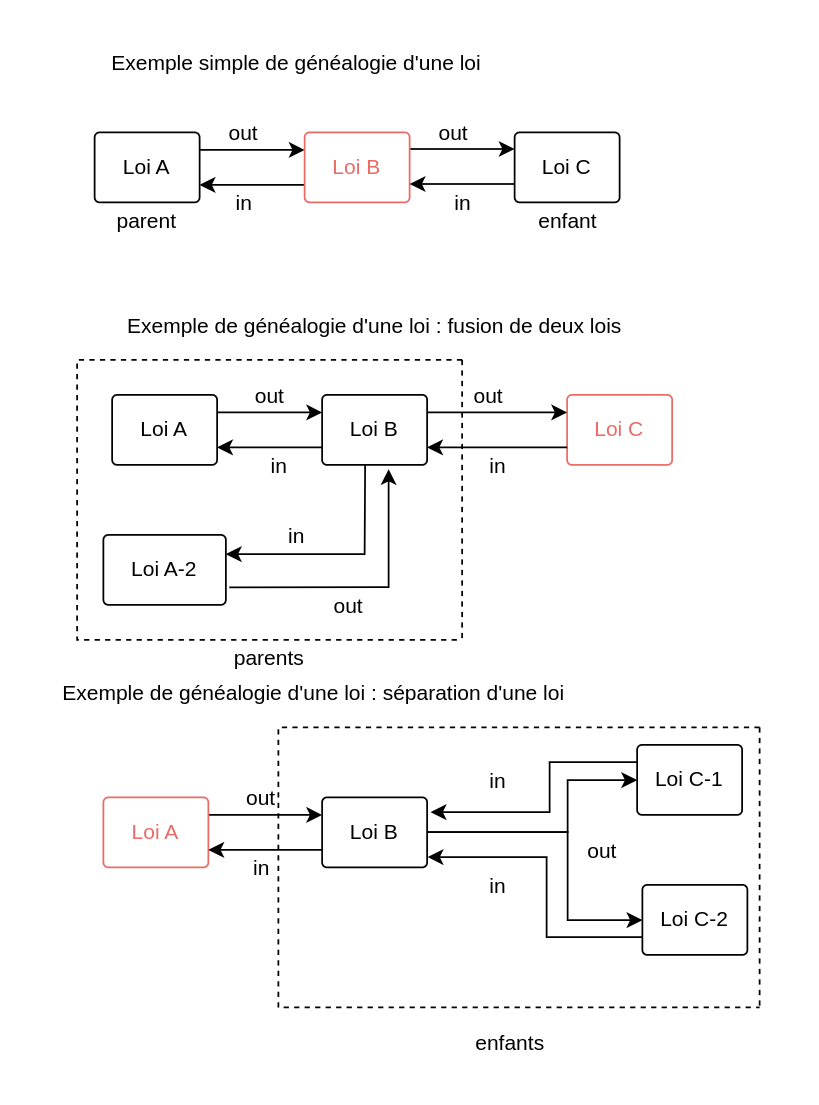
\includegraphics[width=\textwidth]{images/annexe8.png}

\newpage
\subsection*{Recomposition du code virtuel}
Le code virtuel est la recomposition d’un code légal, pour une année donnée entre 1644 et 1911. La recomposition de ce texte de loi présente toutes les lois en vigueur pour l’année choisie, organisées par chapitres et sections. Cette recomposition s’effectue à partir du corpus du projet. 

\subsubsection{Le résultat attendu}
Le code virtuel devra être accessible sur le site en accès libre pour tous les utilisateurs et le résultat doit être accessible rapidement. 

L’utilisateur doit pouvoir entrer l’année de son choix entre 1644 et 1911 et obtenir pour la date choisie une reproduction d’un texte de loi complet qui présente toutes les lois en vigueur pour l’année donnée.

\noindent 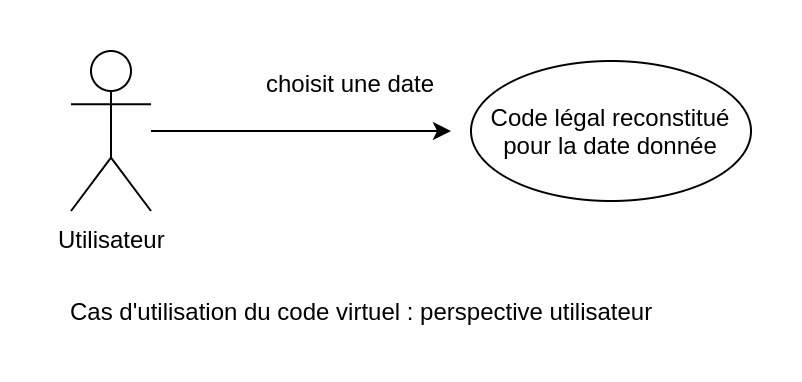
\includegraphics[width=\textwidth]{images/annexe9.png}

Le résultat attendu n’est pas un simple filtrage des lois par date, mais bien une reconstitution artificielle d’un texte de loi. En sortie, le code virtuel doit donc présenter le texte comme s’il avait vraiment été publié, avec un affichage similaire à l’édition en ligne. Il est donc important de conserver la structure du texte de loi (chapitres, sections) et l’ordre des lois (chaque loi secondaire doit figurer sous la loi principale dont elle dépend).

\noindent 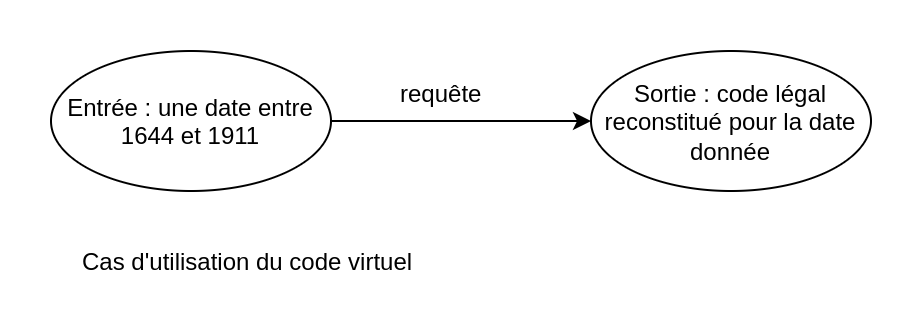
\includegraphics[width=\textwidth]{images/annexe10.png}

\newpage
\section*{Préconisations techniques}
\subsection*{Préparation des données}
\subsubsection{Les données nécessaires}

\textbf{Pour l'édition en ligne}

Pour enrichir les sources afin de répondre aux besoins des chercheurs, les textes de lois doivent notamment être enrichis avec les entités nommées et des commentaires sur les lois (différents des commentaires officiels qui figurent dans les codes légaux). Les entités nommées ont déjà été en partie ajoutées à l’encodage, mais il est pertinent d’ajouter des précisions, notamment des noms de fonction. Ces données sont collectées et accessibles dans les annotations via les fichiers \JSON. 

Pour publier une édition en ligne des codes avec en regard un visualiseur \IIIF, les liens vers les images doivent être intégrés dans l’encodage. Ce lien doit être un accès direct à la ressource. 

Les différents affichages souhaités pour le site sont corrélés à l’encodage des données. Pour afficher les métadonnées d’une loi, il faut intégrer dans les documents, ou dans un document \TEI dédié à cet usage, lesdites métadonnées (avec une référence à l’identifiant \XML de la loi). 

\bigskip
\textbf{Pour le code virtuel}

Pour reconstituer un texte de loi, il faut des bornes chronologiques précises pour chaque loi, afin de pouvoir déterminer quelles lois sont en vigueur pour l’année donnée. Ces données sont disponibles en partie dans les annotations : nous disposons des dates de début de chaque loi. Grâce aux liens d’association dirigée entre les lois, il est possible de déduire la date de fin de chaque loi : une loi prend fin lorsqu’elle est remplacée par une autre. Il faut donc expliciter cette information afin de récupérer pour chaque loi des bornes chronologiques, puis les intégrer à l’encodage. 

Les textes de lois à notre disposition contiennent également des doublons : certaines lois se retrouvent dans plusieurs sources. Il faut donc trouver un moyen de les dédoublonner en leur attribuant un identifiant unique. Cela permettrait de filtrer les lois selon leur identifiant et de n’afficher qu’une seule fois la loi si elle possède des doublons. Les lois qui se retrouvent dans plusieurs codes sont indiquées par les liens d’association entre les lois. \footnote{À propos des liens d’association et d’association dirigée entre les lois, voir l’état des lieux, section \og les liens entre les lois \fg.} Ce système d’identifiant sera également utile pour faire des renvois entre les textes si nécessaire. 

\subsubsection{Échantillon des données}
Un encodage \TEI idéal a été préparé sur un échantillon du \dc (chapitre 6, section 25, \textit{lü} 254 et \textit{tiaoli} 1), afin de présenter ce à quoi les données devront ressembler afin de réaliser le projet. 

\bigskip
\textbf{Les entités nommées}

Pour le balisage des entités nommées, il est recommandé d’utiliser la balise \texttt{<persName>} pour les noms de personne, avec la balise \texttt{<roleName>} si le titre du fonctionnaire est utilisé. 

\noindent 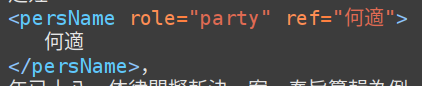
\includegraphics[width=\textwidth]{images/annexe11.png}

Il est également possible de faire dans le \texttt{<teiHeader>} la liste des entités nommées, et de les lister une à une dans la balise \texttt{<person>}. Cela permet de leur attribuer un identifiant unique \texttt{@xml:id} et d’y faire référence dans le corps du texte. Chaque balise \texttt{<person>} contient un attribut \texttt{@role} qui permet de donner le nom de la fonction. Grâce à ce recensement, il est également possible d’ajouter des informations biographiques avec la balise \texttt{<note>}. 

\noindent 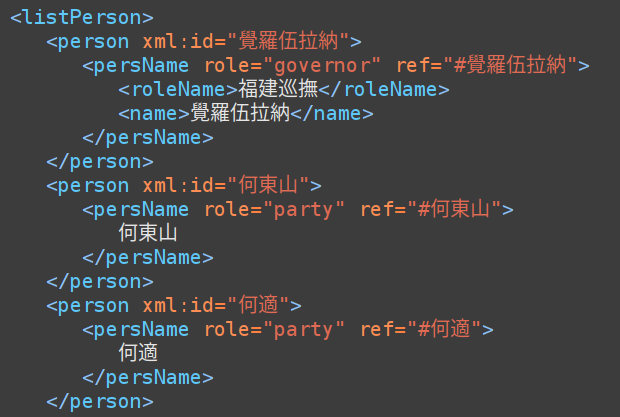
\includegraphics[width=\textwidth]{images/annexe12.png}

Pour les lieux, il est possible d’ajouter un attribut \texttt{@type} (lieu d’application de la loi ou lieu d’origine) et également de faire une liste des lieux, qui contient à minima le nom du lieu et un identifiant unique et éventuellement des informations supplémentaires sur le lieu. Il est également possible de faire correspondre le nom de lieu à l’époque des Qing avec le nom actuel du lieu s’il a changé, de donner des coordonnées géographiques, etc.

\noindent 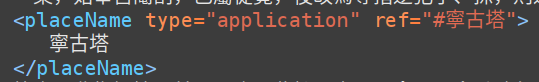
\includegraphics[width=\textwidth]{images/annexe13.png}

Les listes des entités nommées se placent dans le \texttt{<teiHeader>} et contiennent des métadonnées sur ces entités. Cette liste permet aussi d’éviter les erreurs d’encodage car chaque entité nommée est encodée une fois dans le \texttt{<teiHeader>}, puis on se réfère dans l’encodage à l’identifiant \texttt{@xml:id} contenu dans cette liste avec l’attribut \texttt{@ref}. 

\noindent 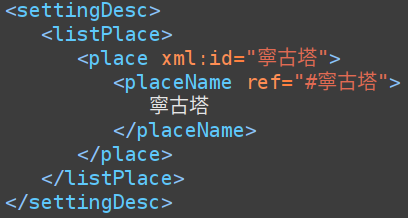
\includegraphics[width=\textwidth]{images/annexe14.png}

\bigskip
\textbf{Les commentaires}

Des commentaires sur les lois peuvent être ajoutés avec la balise \texttt{<note>}. Afin de les distinguer, il convient de leur attribuer un attribut \texttt{@type}. Le nom du type doit correspondre à un mot anglais, par exemple \og official \fg pour les commentaires qui sont rédigés au sein du texte de loi. Les types de commentaires sont déterminés en amont : \textit{official}, \textit{metadata}, etc. Les commentaires de type \textit{metadata} contiennent des métadonnées sur l’origine des lois. 

\bigskip
\textbf{Les liens vers les images}

Afin d’intégrer les images en regard du texte, il est nécessaire d’intégrer le lien de la ressource dans un attribut \texttt{@facs}. Ces liens peuvent se retrouver dans les fichiers \JSON. Le projet n’a pas pour objectif de créer un fac similé interactif, mais simplement de permettre à l’utilisateur de consulter les sources via le visualiseur \IIIF. Les attributs \texttt{@facs} devront donc apparaître sur les balises \texttt{<div>}, la segmentation effectuée permettant d’identifier le début des chapitres, sections et lois. 

\bigskip
\textbf{Les bornes chronologiques}

Afin de pouvoir filtrer pour une année les lois en vigueur, il est nécessaire d’ajouter pour chaque loi une date de début et une date de fin. Pour ajouter les dates en tant qu’attribut sur chaque loi principale et loi secondaire, il est possible d’adapter la \TEI dans l’\ODD afin d’autoriser les attributs \texttt{@notBefore} et \texttt{@notAfter} sur les balises \texttt{<div>}. Les dates sont à récupérer dans les annotations des images.

\bigskip
\textbf{Les identifiants des lois}

Pour pouvoir identifier les lois qui sont présentes dans plusieurs sources, il faudrait un identifiant pour chacune. Une même loi, présente dans plusieurs sources, aurait donc le même identifiant. Il est possible de récupérer cette information via les liens d’association entre les lois qui ont été établis dans Freizo. 

\noindent \includegraphics[width=\textwidth]{images/annexe15.png}

\subsubsection{Étapes de transformation et de validation}
Pour obtenir un document encodé en \TEI à partir des documents \XML du projet \LSC, il est nécessaire de transformer le document \XML grâce à la feuille de style \XSL via le logiciel Oxygen. Les documents doivent ensuite être encodés avec les informations manquantes, en prenant exemple sur l’échantillon. Les données doivent ensuite être validées par l’\ODD, qui contient les règles de validation du schéma choisi pour l’encodage des documents. C’est une étape préalable à l’ajout des documents sur le site. 

Il est également possible d’encoder directement des fichiers en \TEI, auquel cas l’étape de transformation \XSL n’est pas nécessaire. Il suffit d’ajouter les informations aux documents \XML-\TEI de référence, ou bien d’encoder un nouveau document en \TEI en suivant la documentation. 
\newpage
\noindent 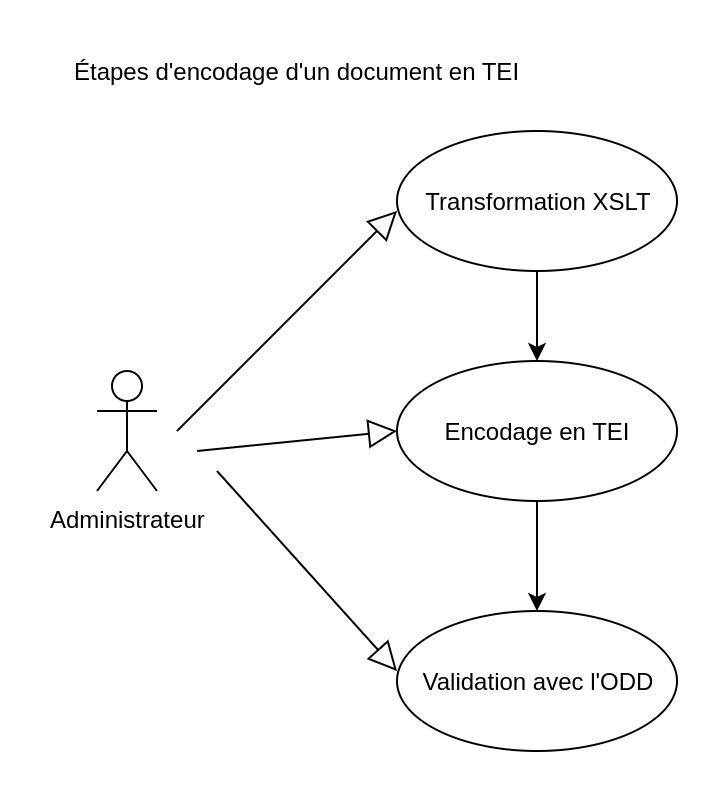
\includegraphics[width=\textwidth]{images/annexe16.png}

Pour valider un document avec l’\ODD, il faut lier le fichier \href{https://sharedocs.huma-num.fr/wl/?id=yHHcUPKWyusazIZqWVLgtbZI7J65OaLA&path=ODD%2Fout&mode=grid}{ODD_COREL.rng} dans le document \TEI, comme ceci : 

\noindent 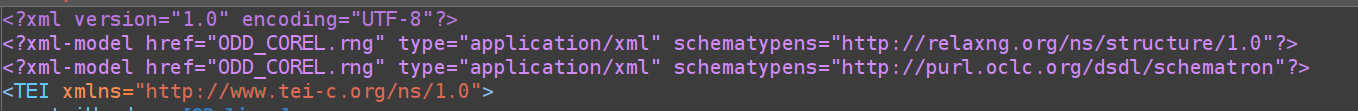
\includegraphics[width=\textwidth]{images/annexe17.png}

L’\ODD permet ensuite à Oxygen de signaler les erreurs à l’utilisateur, avec plusieurs niveaux d’importance. Les erreurs rouges signalent un problème d’encodage bloquant pour le projet, par exemple l’absence de données comme les dates des lois ou les identifiants \texttt{@xml:id}. Les erreurs oranges signalent des erreurs moins importantes, comme par exemple l’absence de l’attribut \texttt{@facs}, qui est nécessaire pour proposer la numérisation des codes sur le site, mais qui n’empêche pas son bon fonctionnement.
\newpage

\section*{Outil envisagé}
\href{https://teipublisher.com/exist/apps/tei-publisher/doc/documentation.xml?odd=docbook&view=div&id=selected-use-cases&hash=3.6.5#introduction}{\tp} est un outil dédié à la publication de textes encodés en \XML-\TEI en ligne. Il s’appuie sur un système de gestion de base de données \XML, eXist-db. L’objectif de \tp est d’offrir un framework permettant de publier des éditions en ligne avec le moins de code possible. Il offre donc une interface graphique qui permet de publier rapidement et simplement des textes, mais permet aussi un grand niveau de personnalisation. C’est un outil largement utilisé pour la publication de données en \TEI, comme par exemple pour les projets \textit{Démêler le Cordel} de l’Université de Genève ou \textit{Discholed} de l’INRIA. \tp est donc un outil déjà éprouvé par une communauté pour l’édition scientifique numérique, comme le souhaite le projet. 

Cet outil répond aux besoins du projet \COREL car il permet de publier rapidement des données \TEI, en interface graphique. Tout se fait via l’application \tp. De plus, c’est un outil open-source et bien documenté, utilisé par de nombreux projets, ce qui permet d’avoir des exemples sur lesquels s’appuyer. \tp permet aussi de personnaliser son application en modifiant le code en \HTML ou XQuery. Il est également possible d’utiliser des web components.

Si \tp offre une interface graphique pour la publication, cela nécessite tout de même une bonne connaissance des langages \XML et du développement web, notamment pour la modification de l’\ODD via \tp. De plus, pour une application plus développée, comme pour la création du code virtuel, le recours à la personnalisation sera probablement nécessaire et demande également d’utiliser les langages \XML (\XML-\TEI, XQuery, \ODD…). 

\newpage
\section*{Maintenance et hébergement}
Pour l’hébergement, le projet envisage trois options : un hébergement par le porteur administratif du projet, le Collège de France, un hébergement sur les serveurs de l’École Française d’Extrême-Orient, ou bien un hébergement sur les serveurs de l’IR Huma-Num. 

Si un hébergement sur les serveurs d’Huma-Num est envisagé, certains pré-requis doivent être respectés. Huma-Num propose l’hébergement de sites web pour diffuser des données de projet de recherche, mais la maintenance n’est pas incluse. La maintenance corrective du site et la mise à jour est donc aux frais du projet \COREL. Ce choix d’hébergement va de pair avec la possibilité de déposer les numérisations du projet sur Nakala. 

Pour être hébergé par Huma-Num, il est nécessaire d’indiquer sur la page d’accueil du site que l’IR Huma-Num est l’hébergeur. Le gestionnaire du site doit également demander l’inscription dans l’annuaire des sites web hébergés par Huma-Num. Toutes les données et métadonnées du site doivent être interopérables, dans un format pérenne \footnote{La \TEI fait partie des formats préconisés.} et permettre le moissonnage via le protocole \oai. Un engagement de mise à jour durant toute la vie du site est exigé. 

La maintenance du site web sera assurée par Vincent Paillusson. Cette maintenance sera corrective et prendra en charge les mises à jour du site, ainsi que les corrections d’éventuels disfonctionnements. 

\newpage
\section*{Calendrier prévisionnel}
Le calendrier prévisionnel du projet a été établi à partir d’une carte mentale des étapes restantes dans le projet. \footnote{Voir les annexes}

\newpage
\begin{center}
    \begin{tabularx}{0.9\textwidth}{| >{\centering\arraybackslash}X |
    >{\centering\arraybackslash}X |
    >{\centering\arraybackslash}X |}
    \hline
    N° de tâche & Libellé & Prérequis  \\
    \hline
    A & \textbf{Préparation des données} & \\
    \hline
    A1 & Fichiers \JSON complet (liens entre les lois, URL, dates, identifiants) - prestataire & Prestation Data Futures \\
    \hline
    A2 & Intégrer les données .json dans le .xml (url, xml:id, dates, entités nommées) & A1 \\
    \hline
    A3 & Intégrer des données supplémentaires dans le .xml (commentaires, métadonnées) & \\
    \hline
    B & \textbf{Édition en ligne} & \\
    \hline
    B1& Édition des codes (.xml > TEI Publisher) &A \\
    \hline
    B2 & Ajout de pages supplémentaires (.docx > TEI Publisher) & \\ 
    \hline
    C & \textbf{Code virtuel} & \\
    \hline
    C1 & Mapping des données manquantes dans le Duli Cunyi - prestataire & Prestation DataFutures \\
    \hline
    C2 & Compilation XML à partir du Duli Cunyi de toutes les lois &A1, C1 \\ 
    \hline
    C3& Requête XQuery pour filtrer les données par date & A1, A2 au minimum, éventuellement C1 \\
    \hline
    C4 & Paramétrage de l'affichage (via TEI Publisher ou custom) & C3 \\
    \hline
\end{tabularx}

\begin{tabularx}{0.9\textwidth}{| >{\centering\arraybackslash}X |
    >{\centering\arraybackslash}X |
    >{\centering\arraybackslash}X |}
    \hline
     D & \textbf{Visualisation} & \\
    \hline
    D1& Code JavaScript (créer la visualisation à partir du .json) & A1 \\
    \hline
    D2 &Intégrer les visualisations à l’édition en ligne & D1, B \\
    \hline
    E & \textbf{Référencement et interopérabilité} & \\
    \hline
    E1 & OAI-PMH & A, B, C, D \\
    \hline
    E2 & Référencer les données dans Isidore & A, B, C, D \\
    \hline
    E3 & Déposer les images sur Nakala & \\
    \hline
    F & \textbf{Phase de tests du site web} & A, B, C, D \\
    \hline
    F1 & Tests et corrections & \\
    \hline

\end{tabularx}
\end{center}

\begin{landscape}
    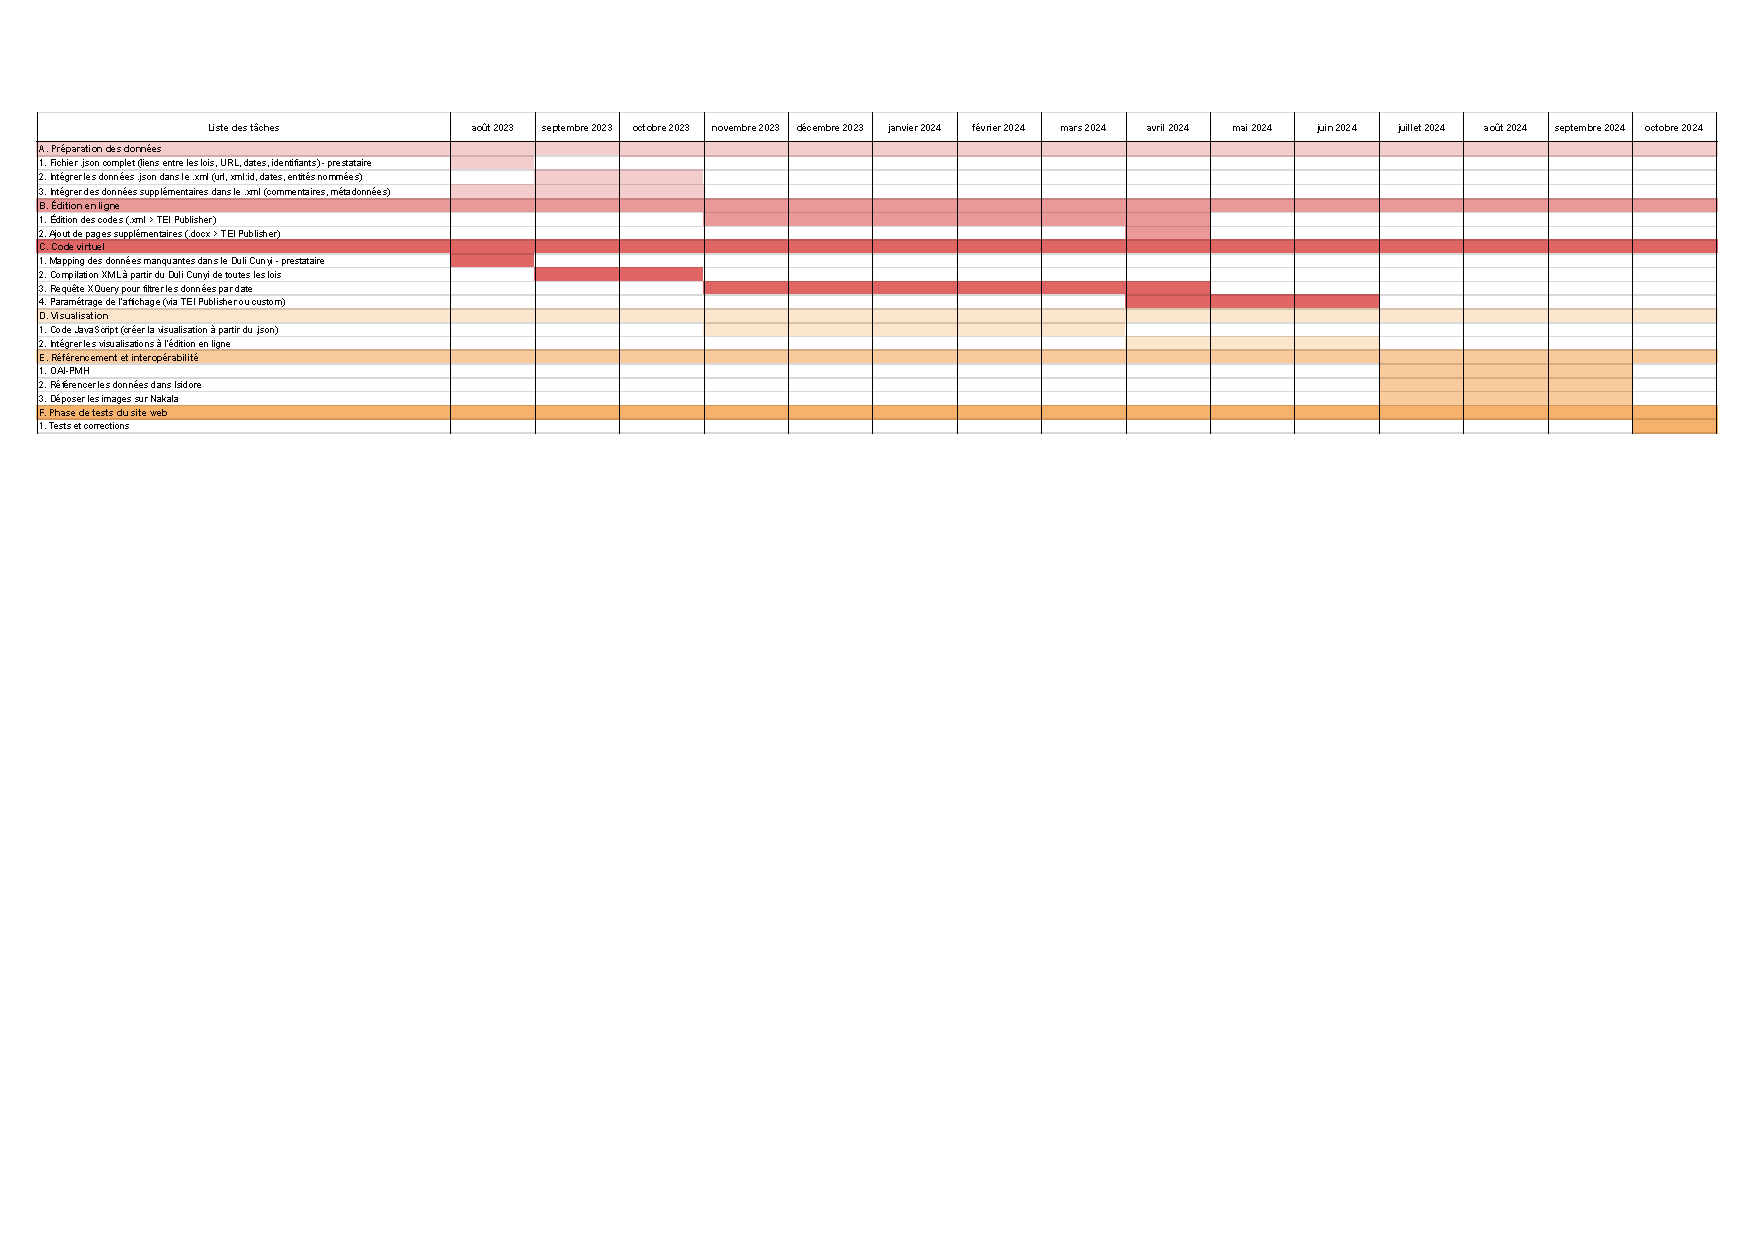
\includepdf[page={1},angle=90]{annexes/calendrier.pdf}
    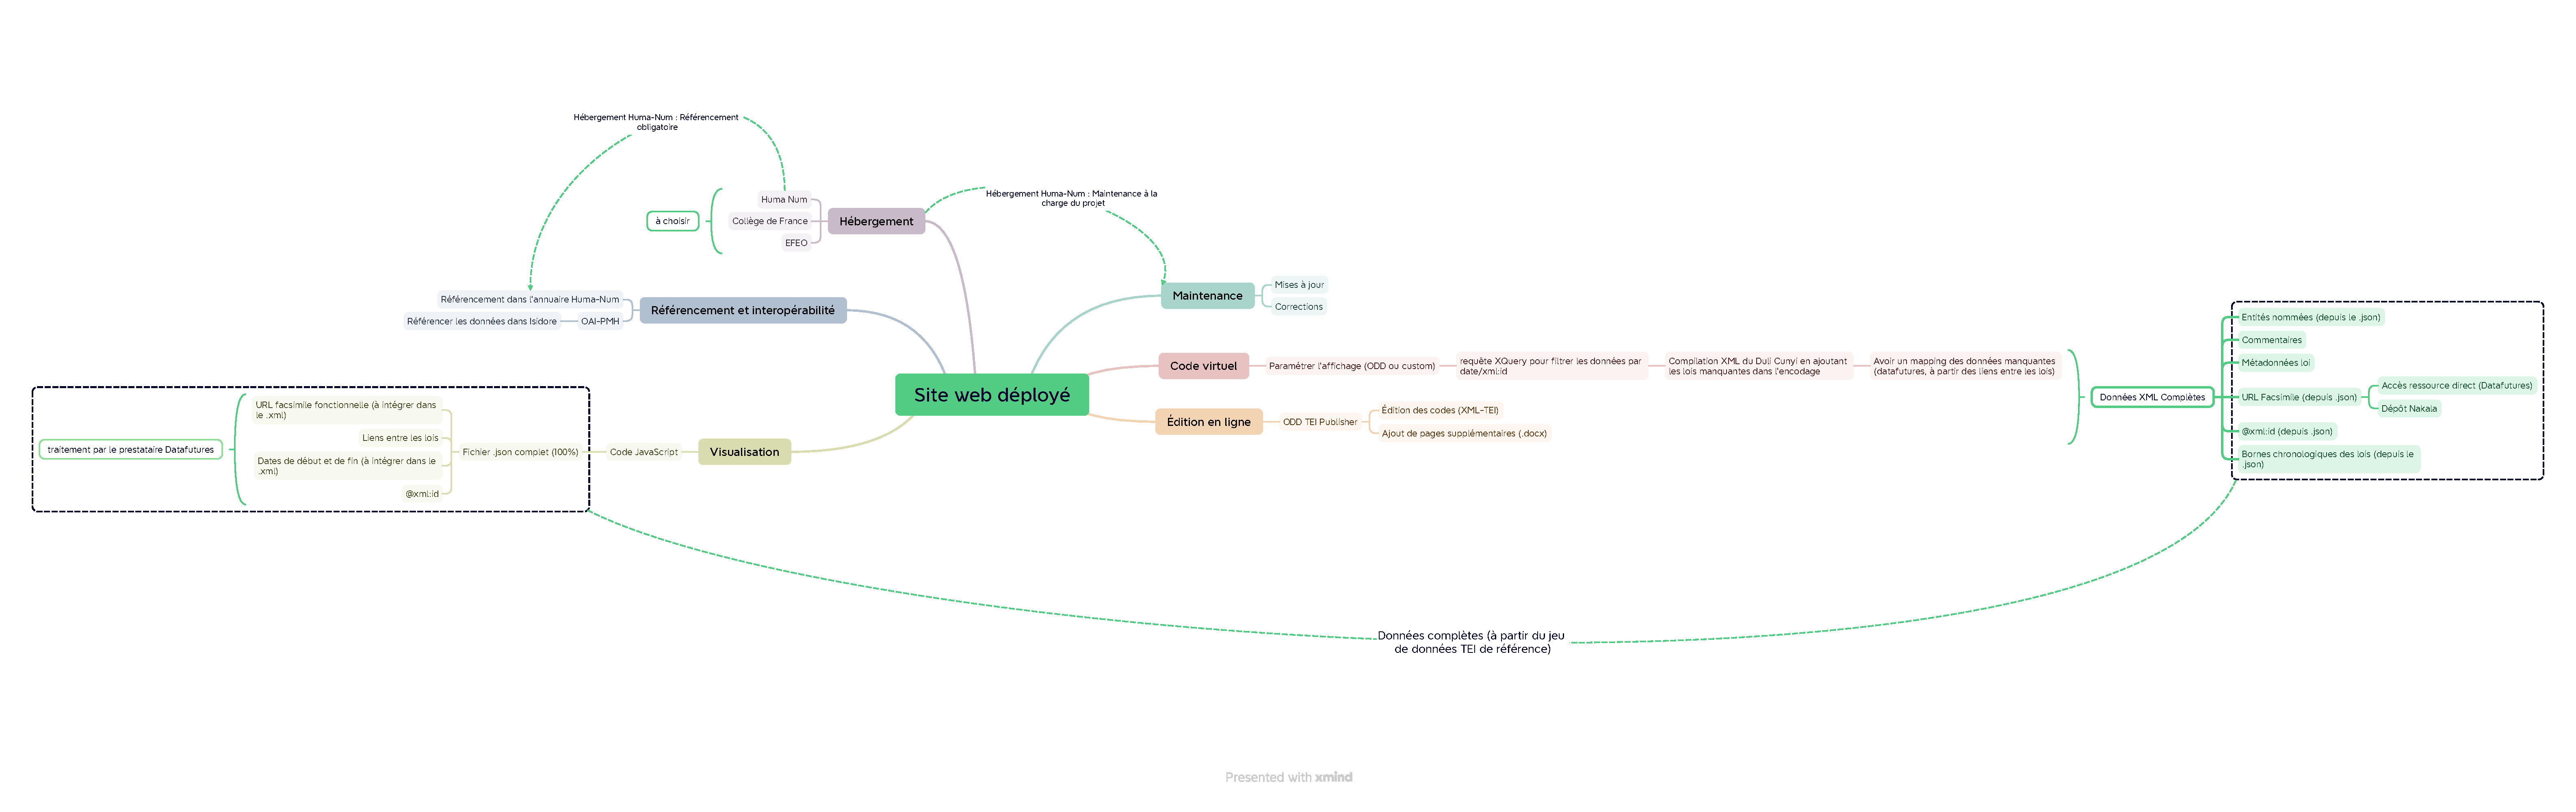
\includepdf[page={1}, angle=90]{annexes/mindmap.pdf}
\end{landscape}

\newpage
\section*{Maquettes}
\noindent 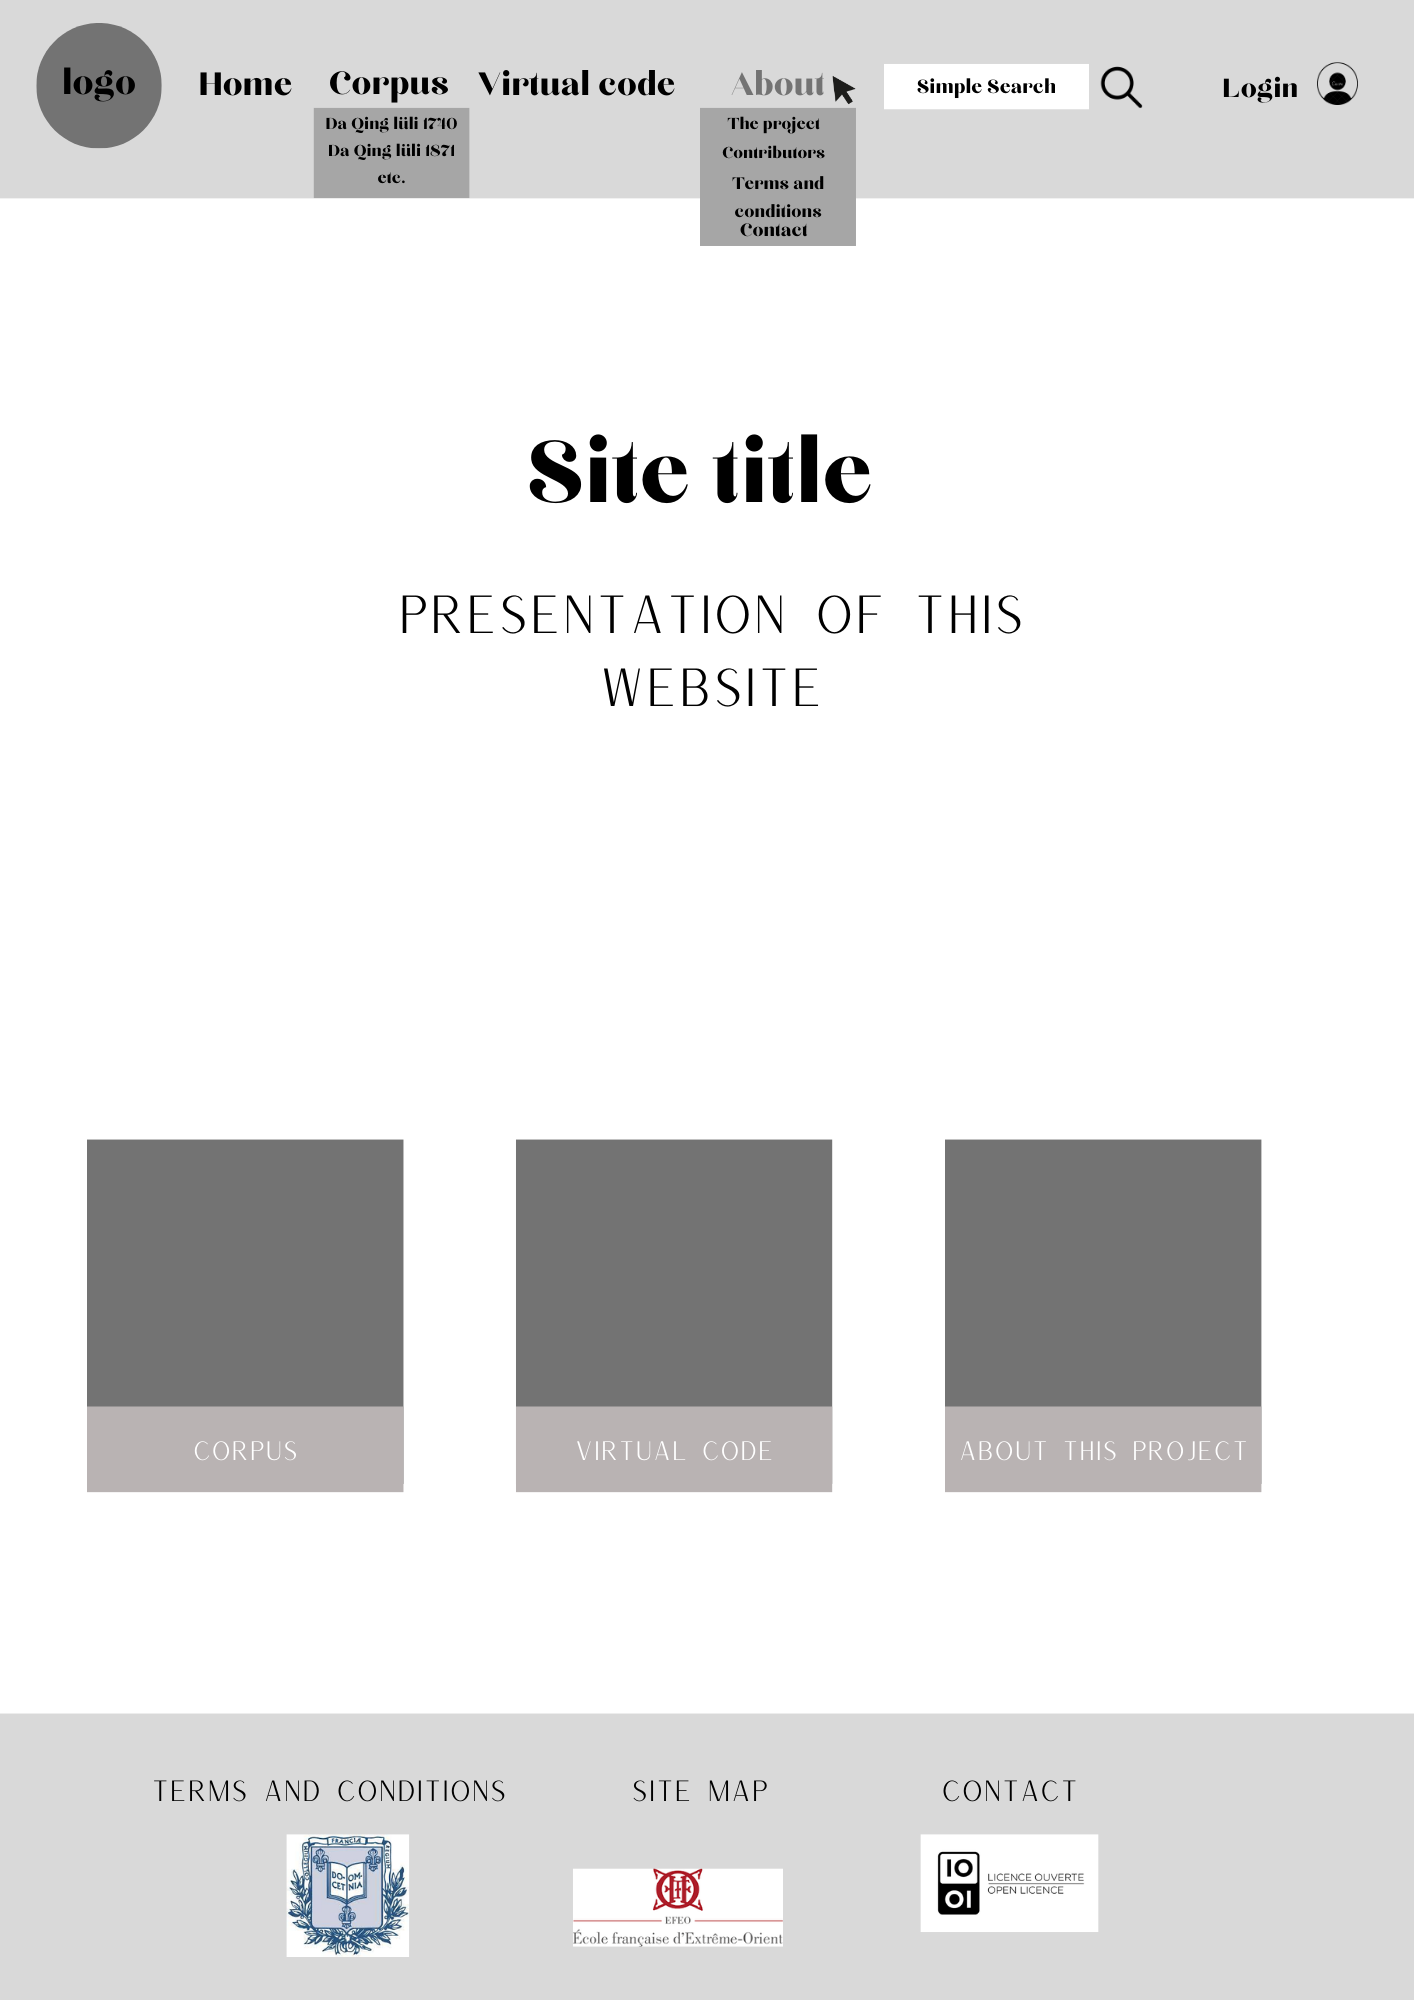
\includegraphics[width=\textwidth]{annexes/1 - Accueil.png}
\noindent 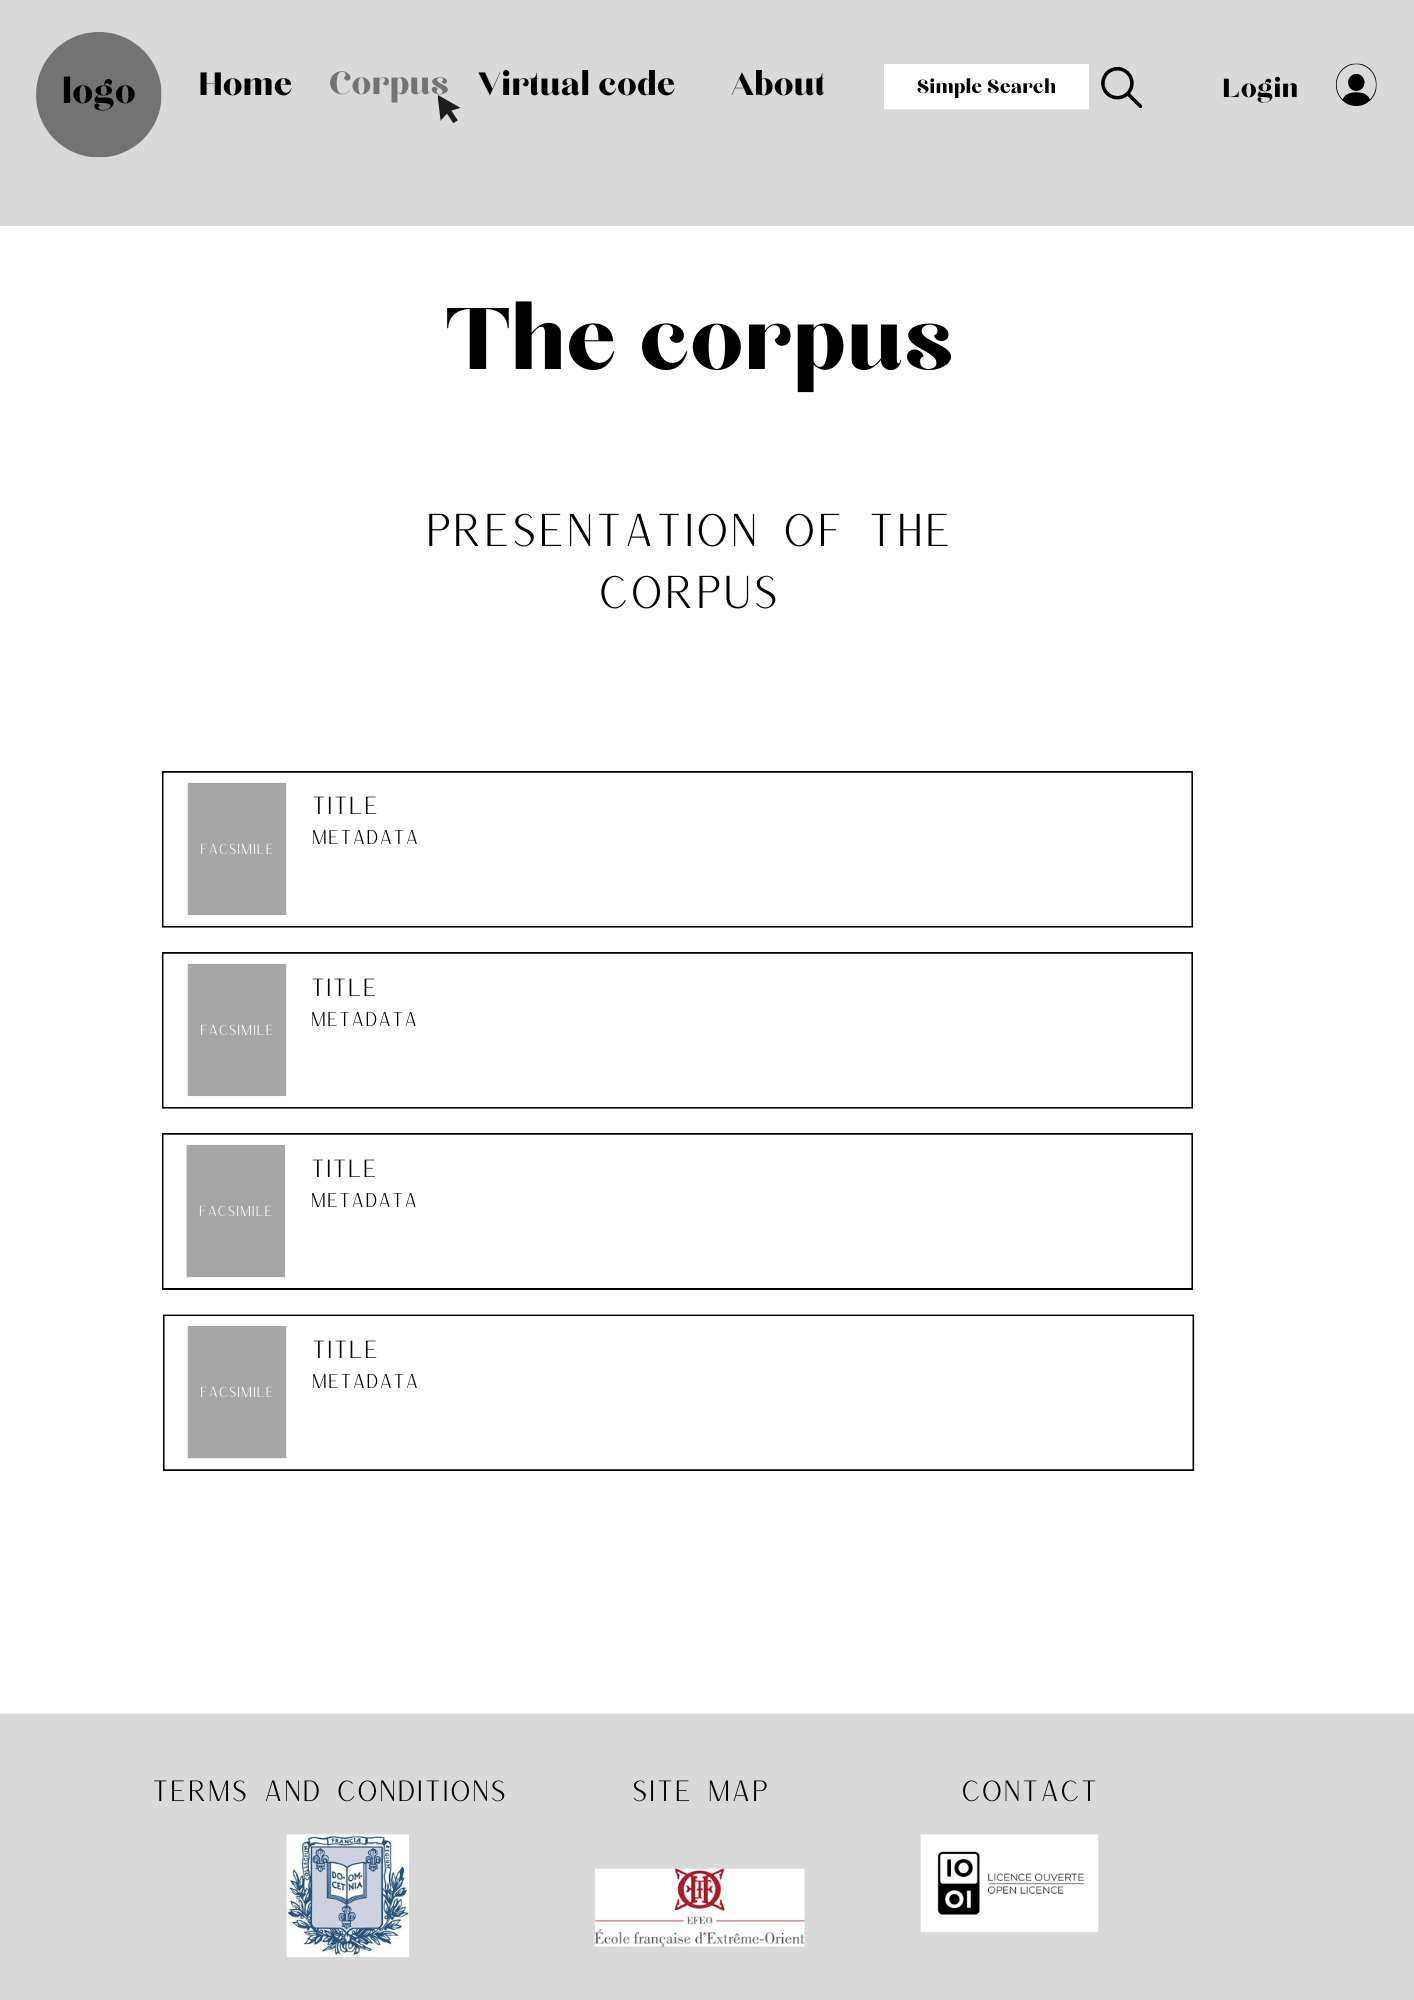
\includegraphics[width=\textwidth]{annexes/2-Corpus.png}
\noindent \includegraphics[width=\textwidth]{annexes/3 - Édition en ligne _ commentaires.png}
\noindent 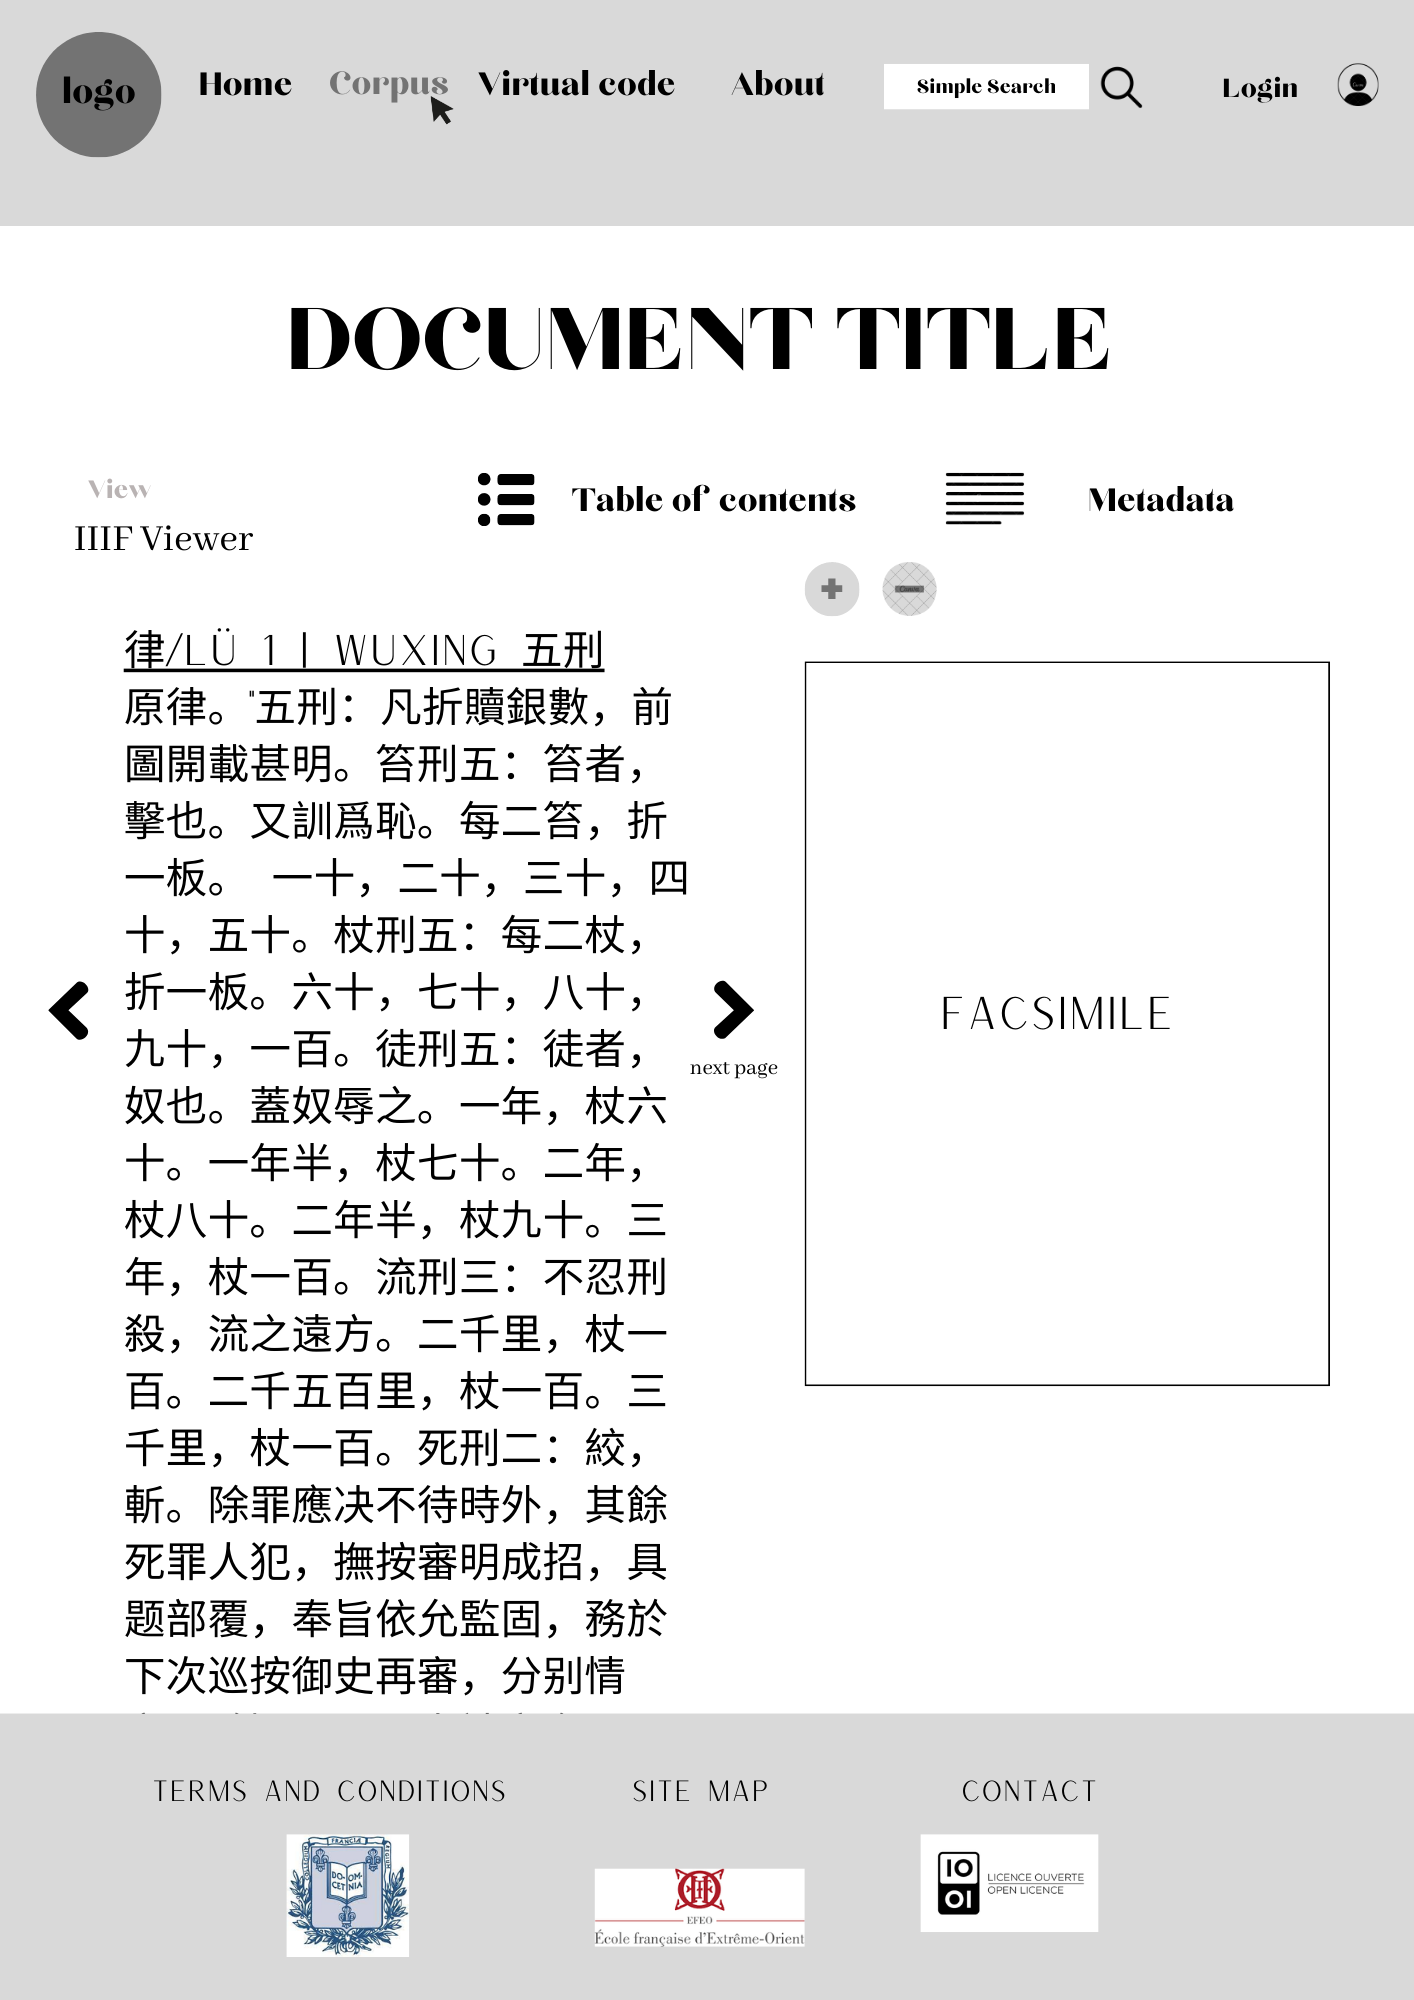
\includegraphics[width=\textwidth]{annexes/4 - Édition en ligne _ fac similé.png}
\noindent 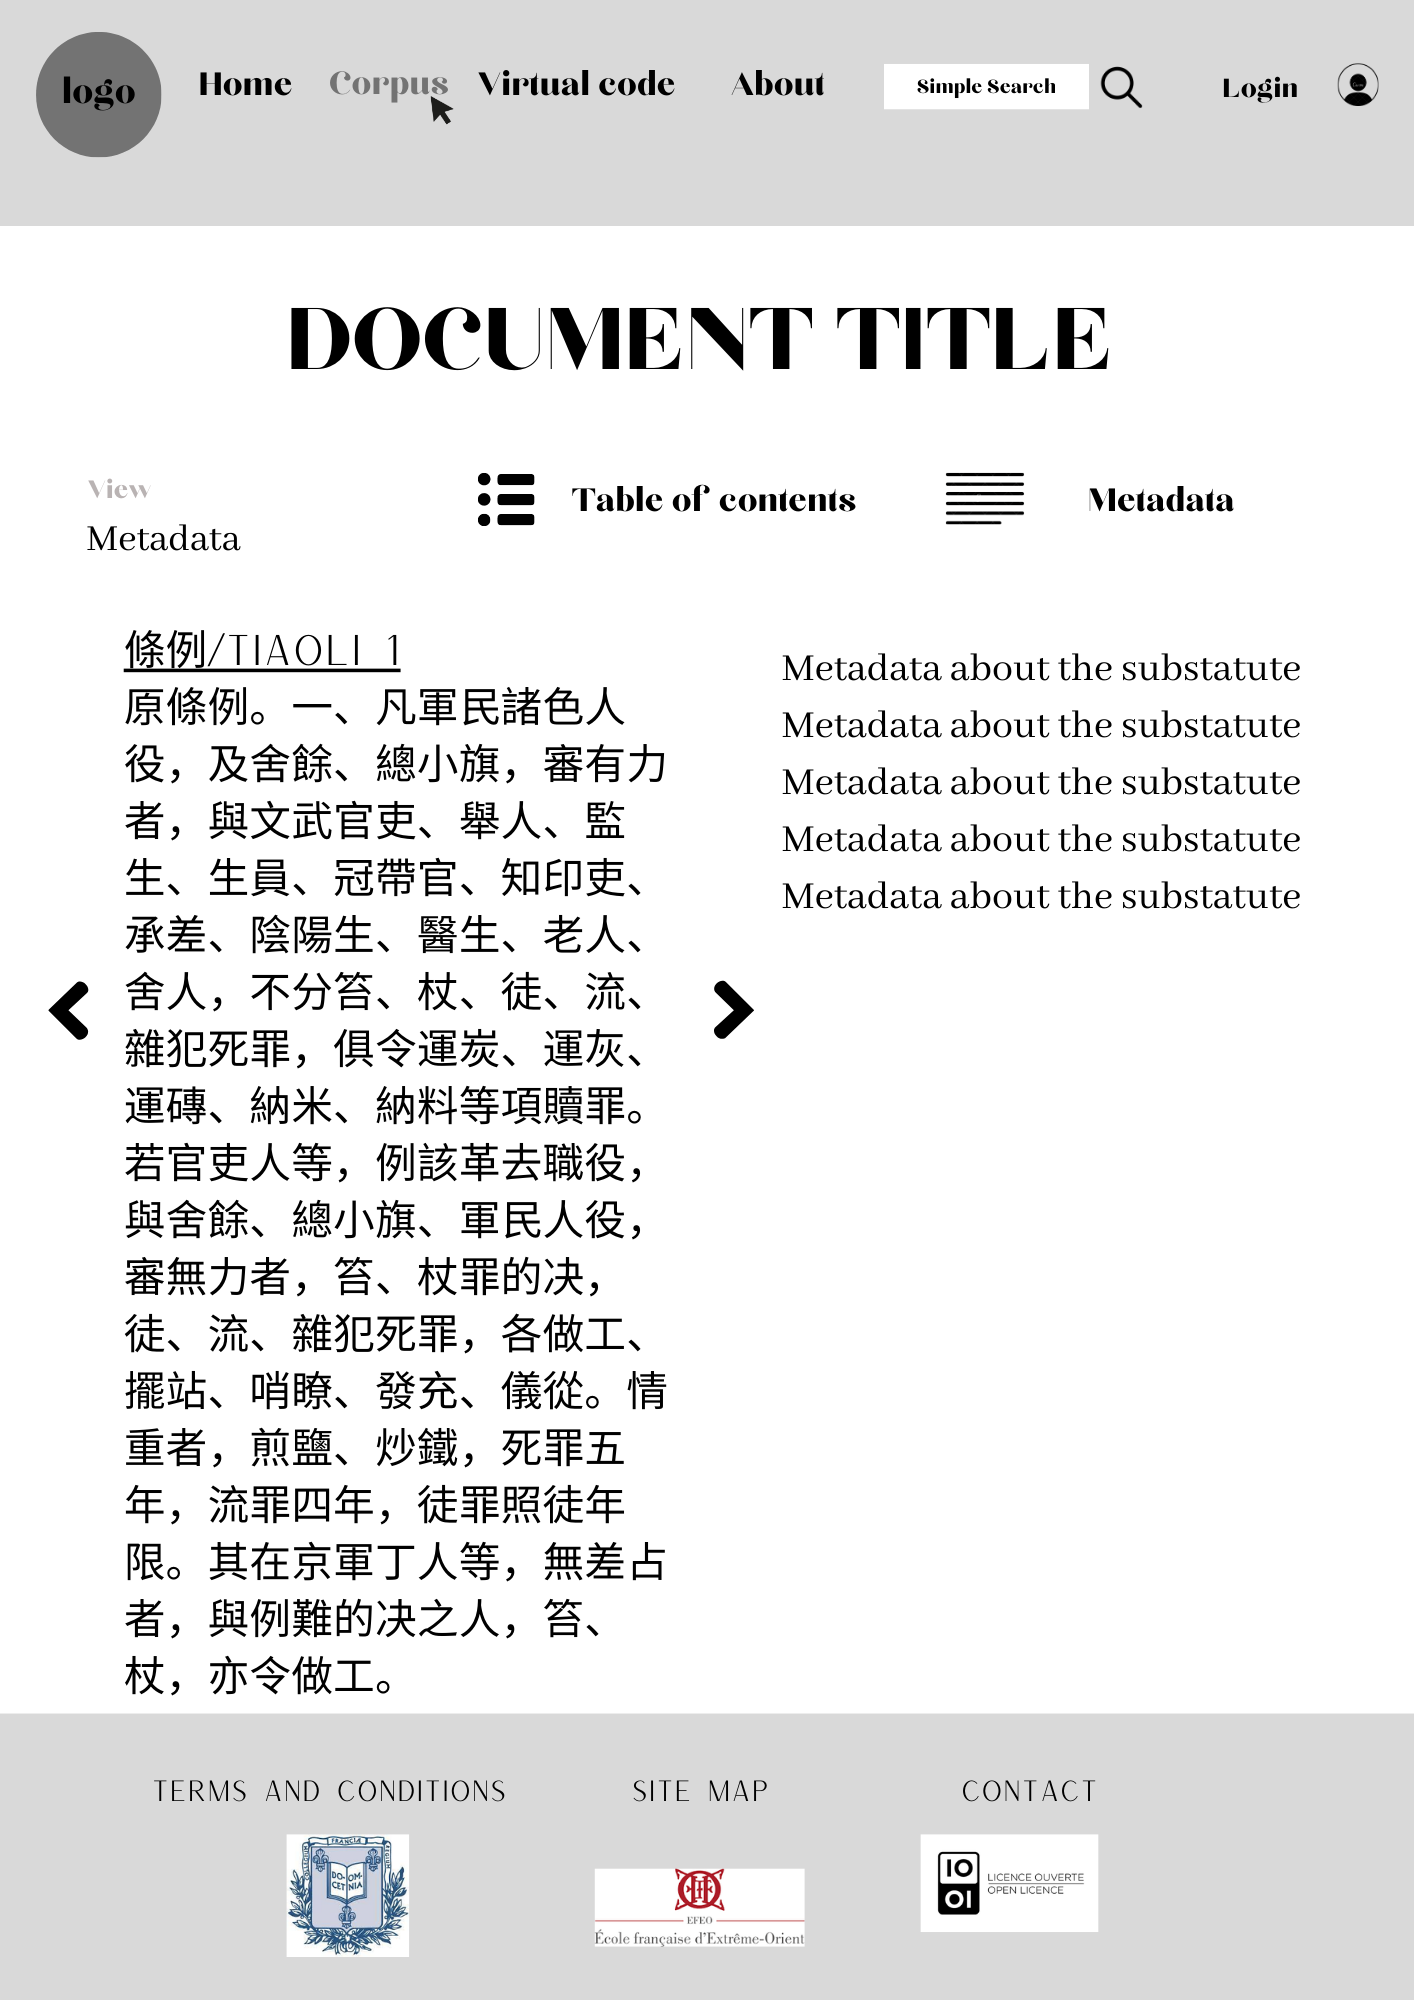
\includegraphics[width=\textwidth]{annexes/5 - Édition en ligne _ métadonnées.png}
\noindent 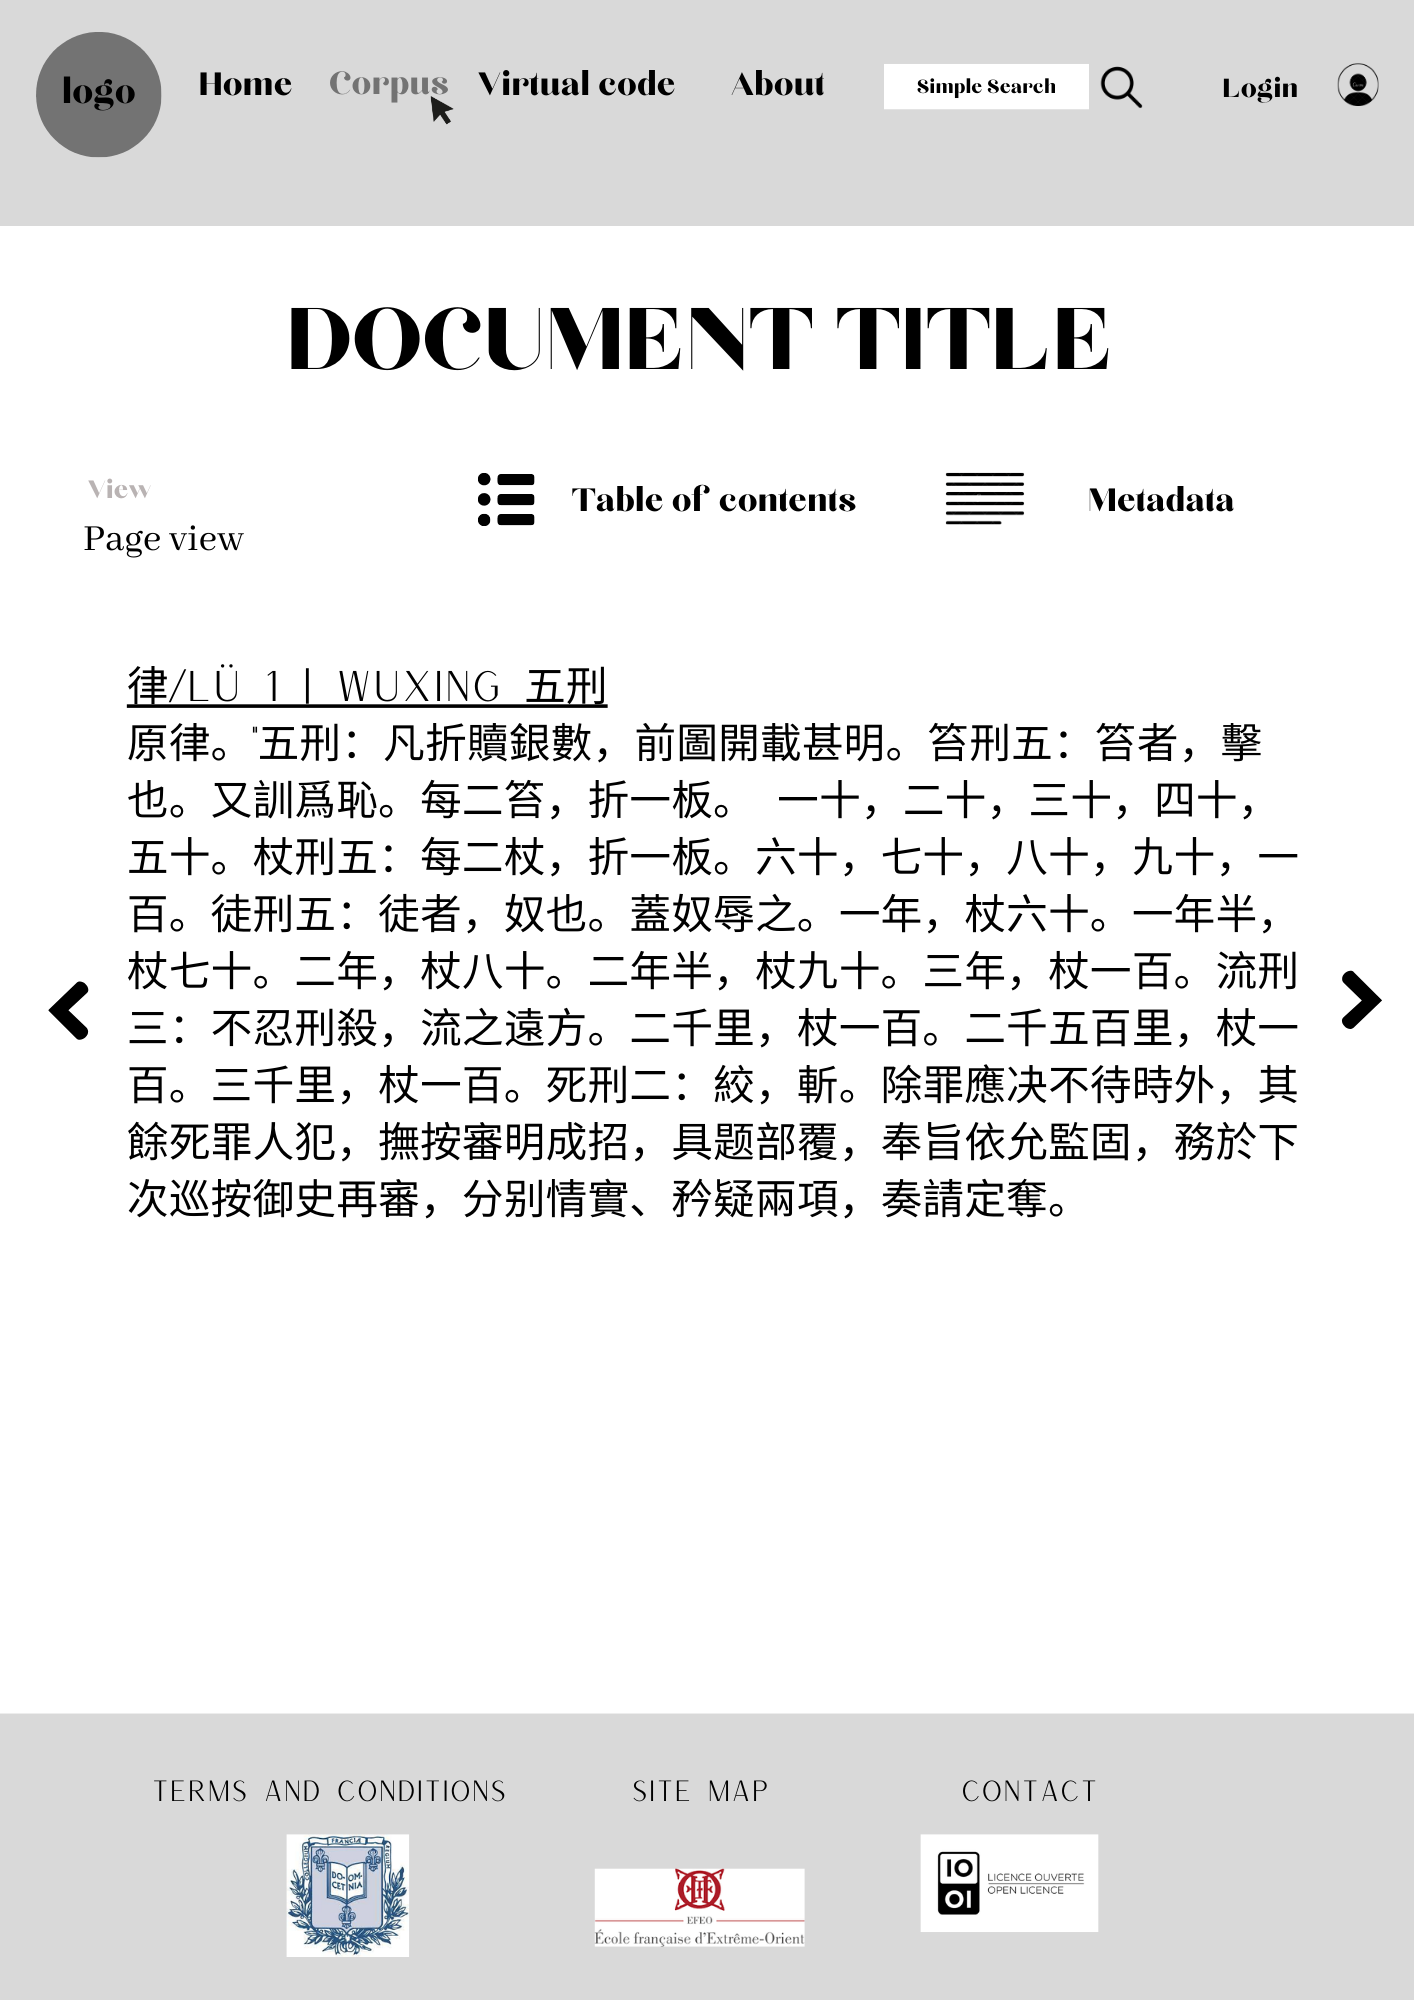
\includegraphics[width=\textwidth]{annexes/6 - Édition en ligne _ texte paginé.png}
\noindent 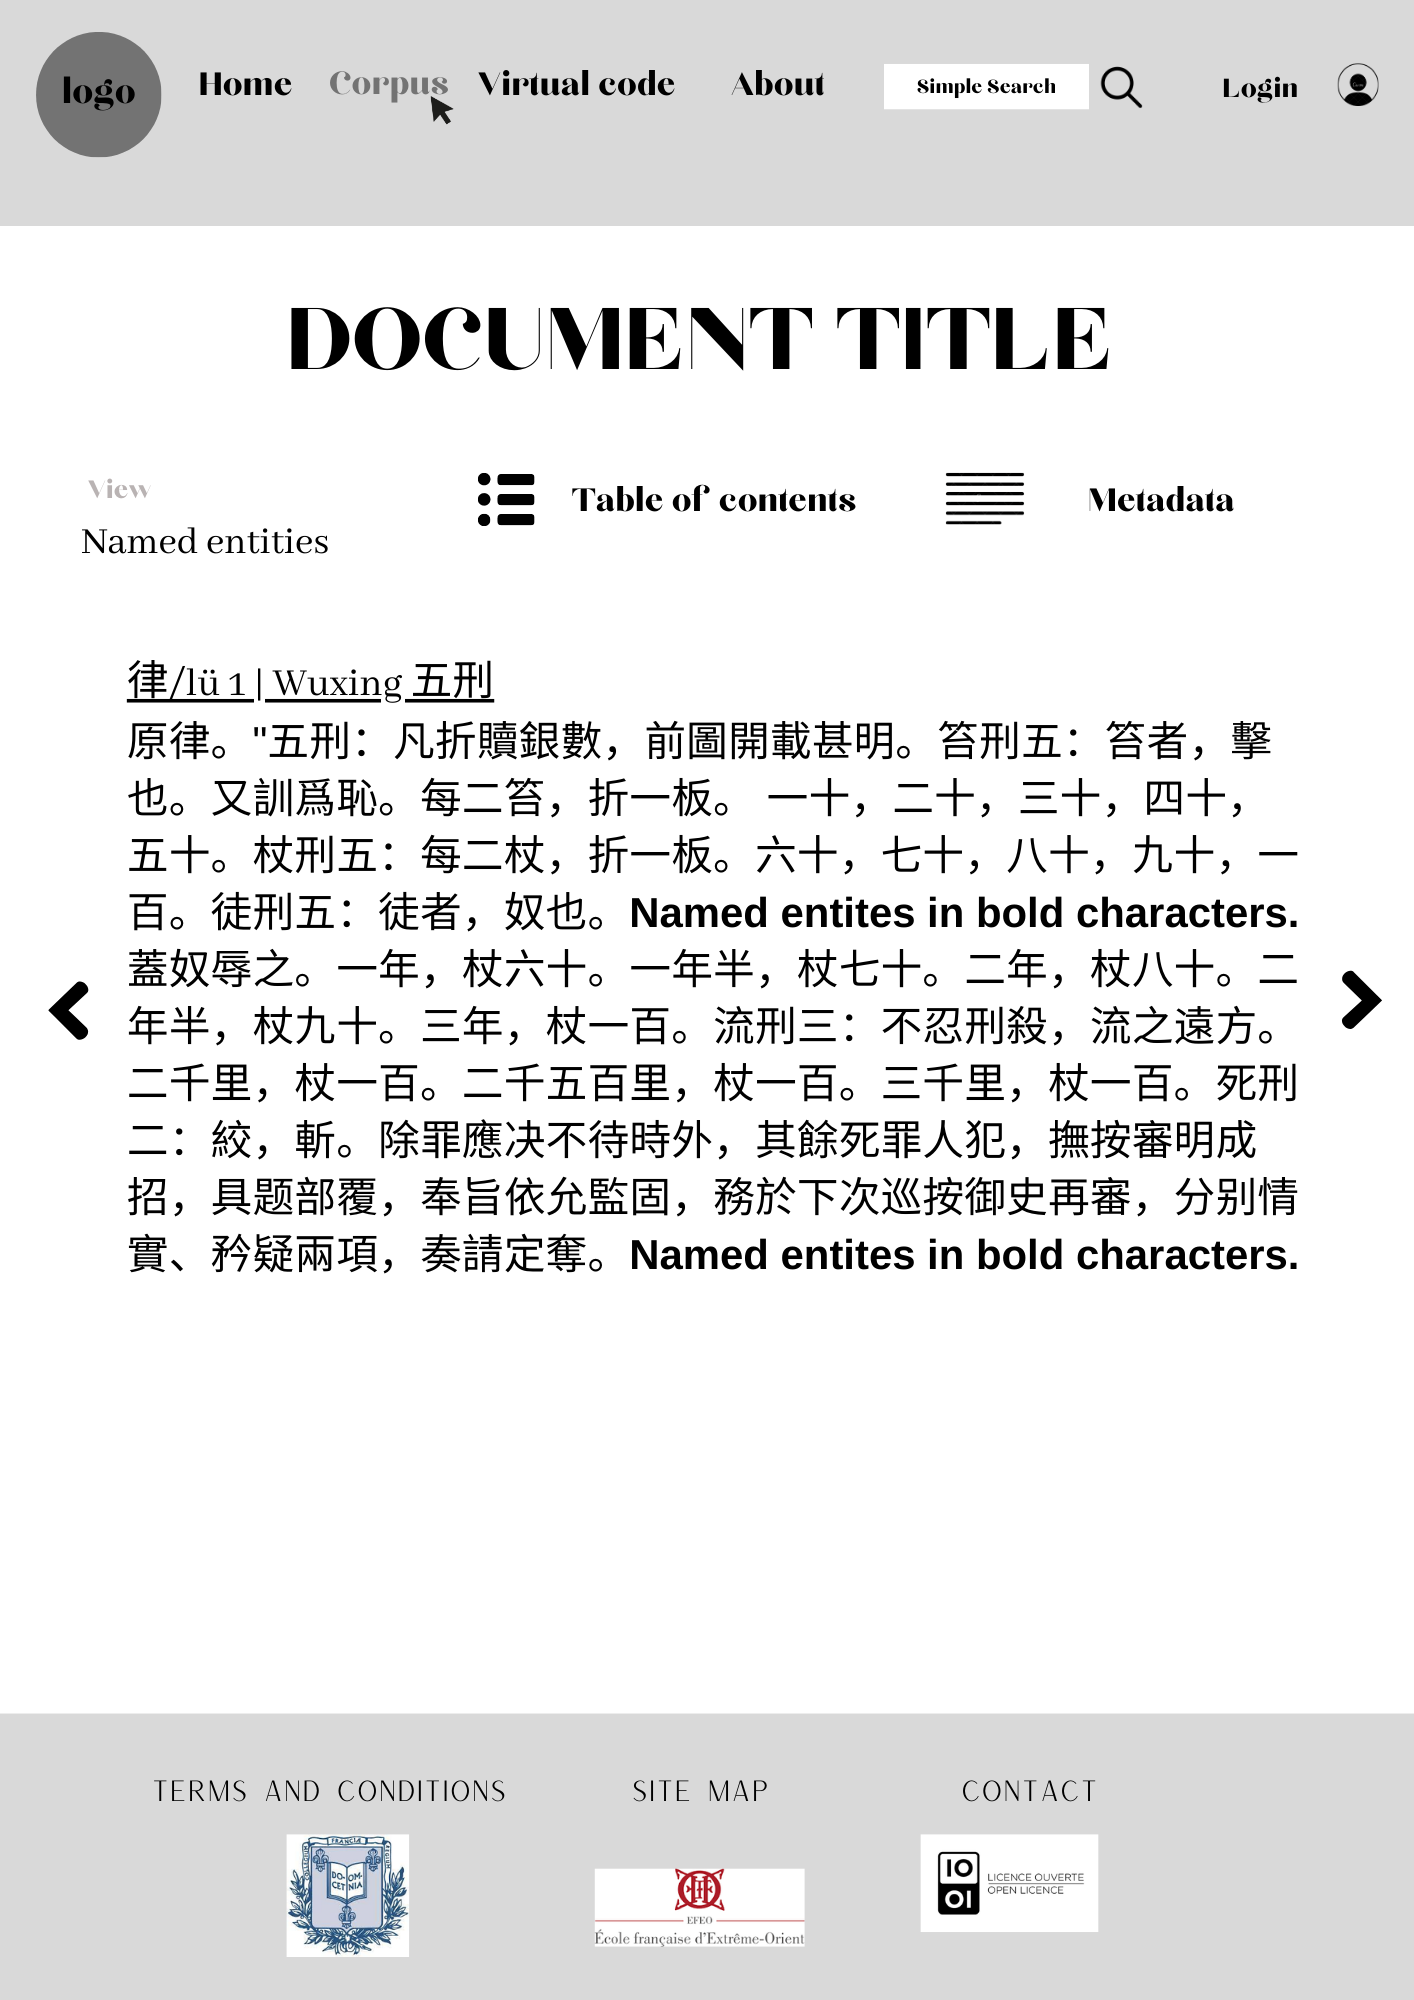
\includegraphics[width=\textwidth]{annexes/7 - Mode _ entités nommées.png}
\noindent 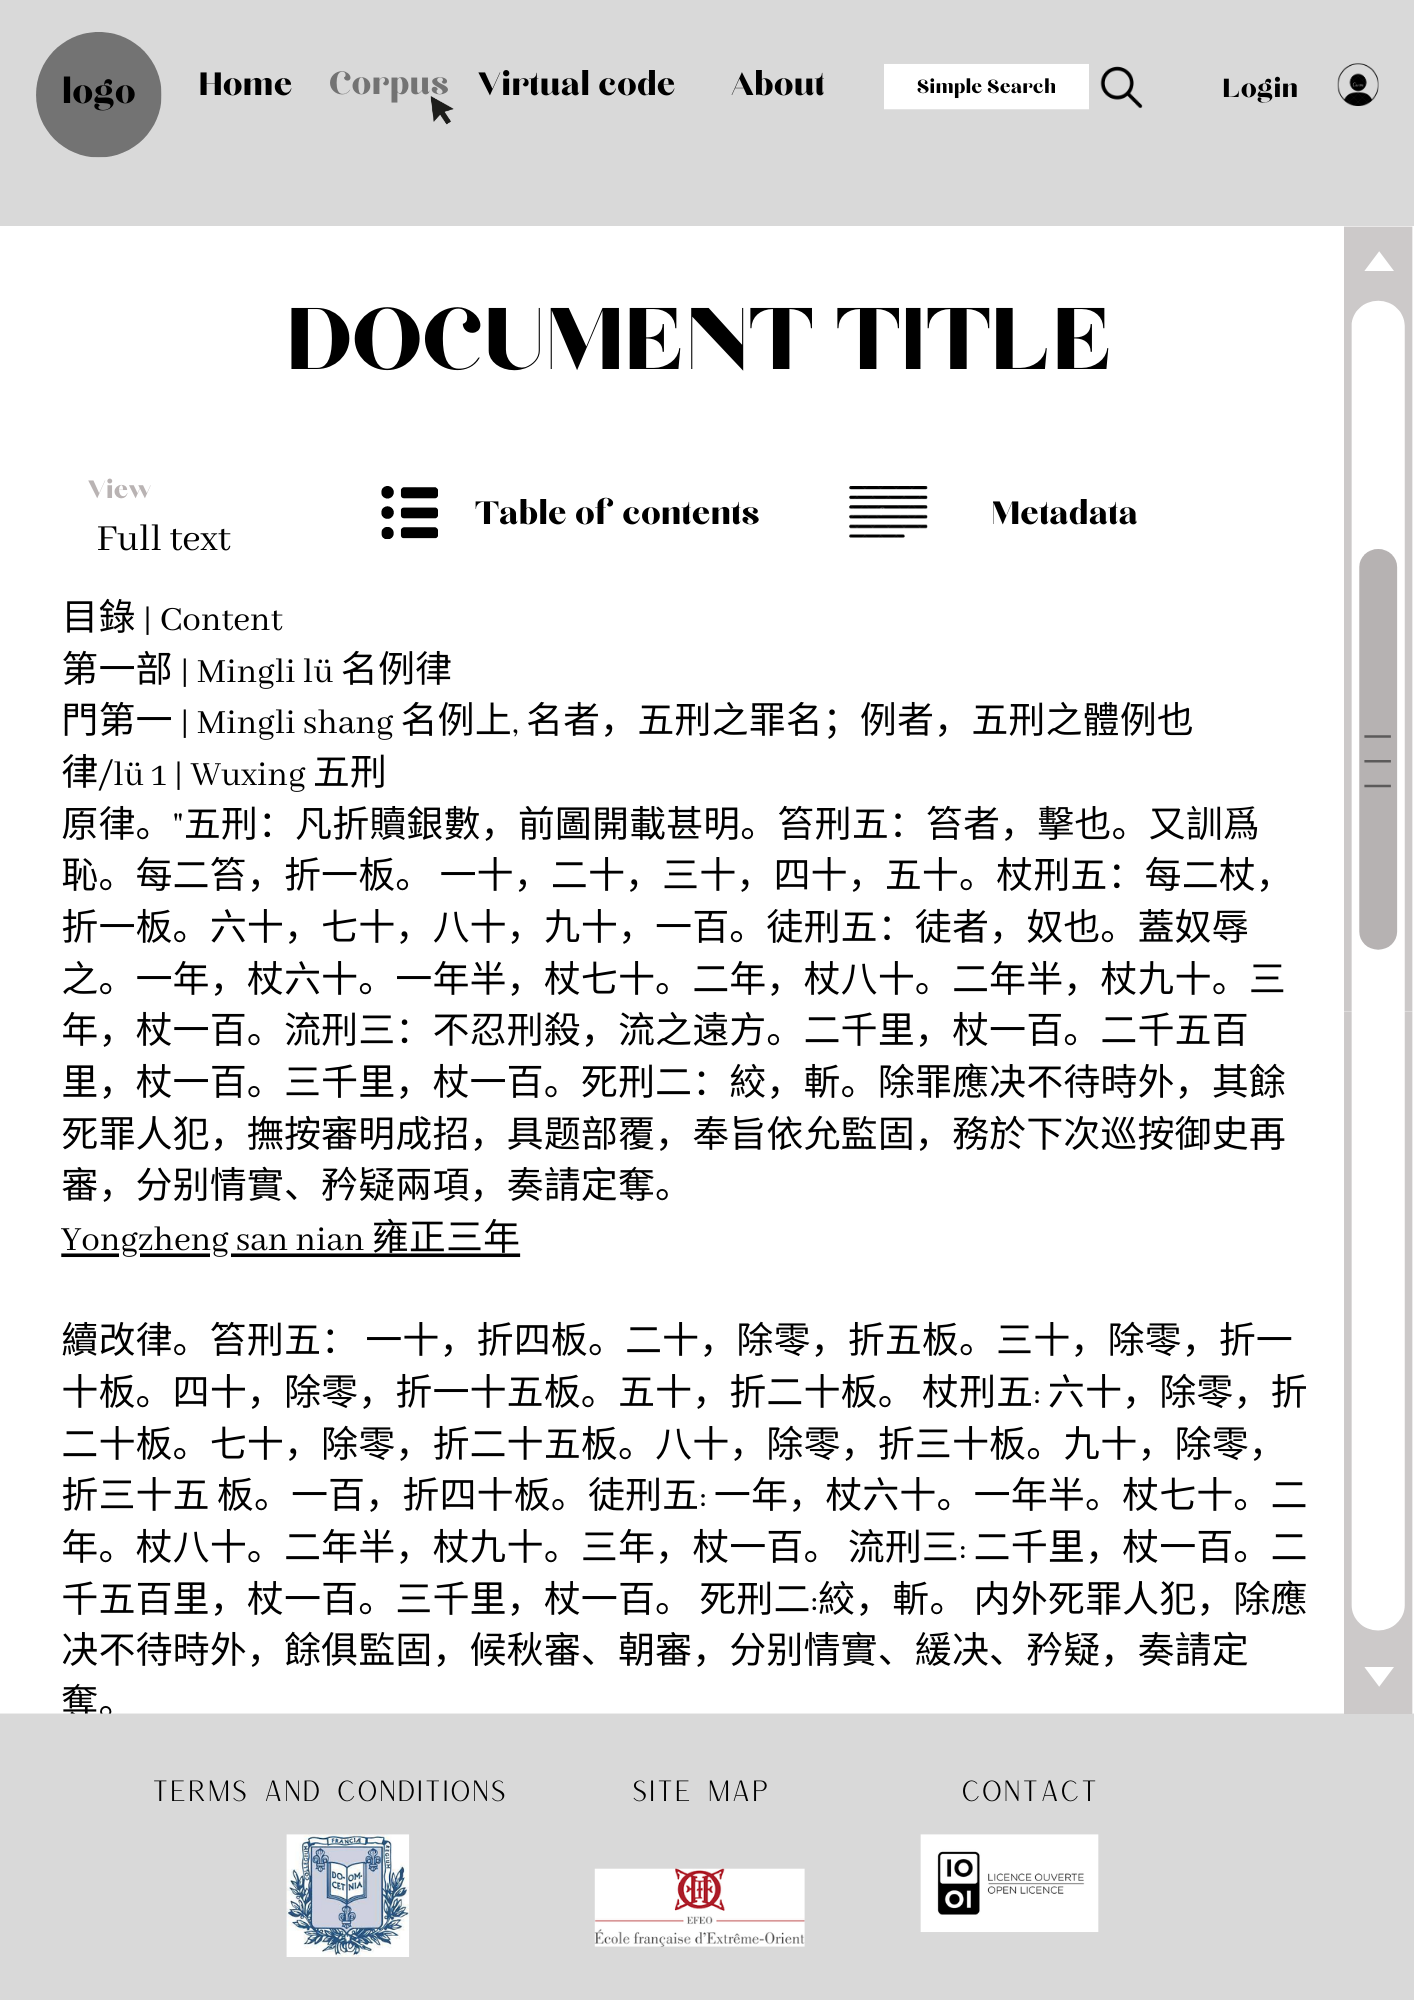
\includegraphics[width=\textwidth]{annexes/8 - Edition en ligne_Texte continu.png}
\noindent 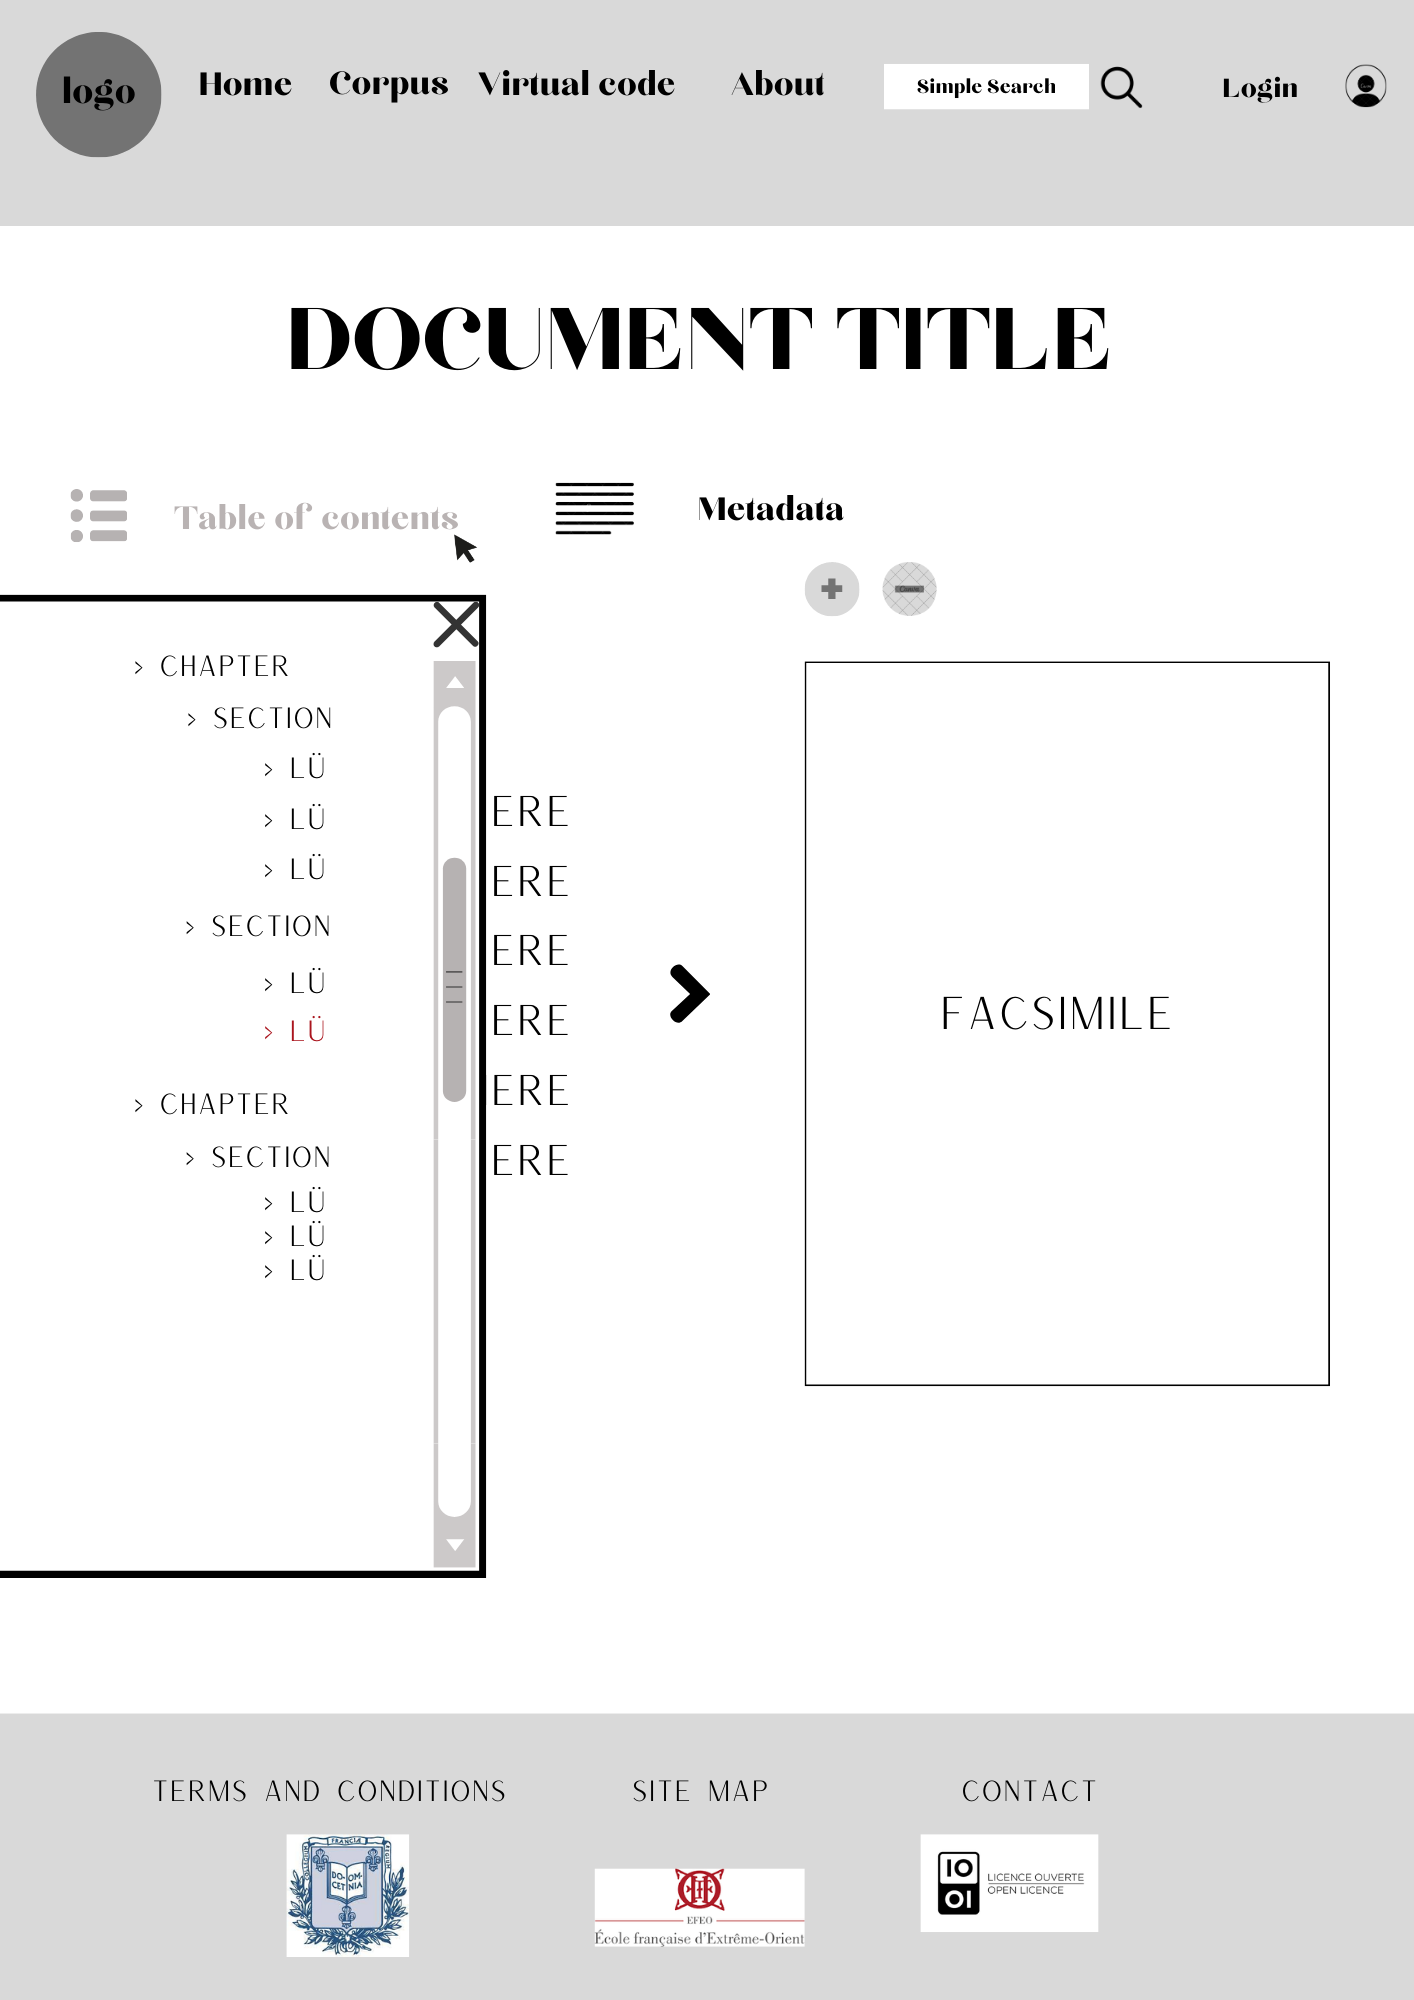
\includegraphics[width=\textwidth]{annexes/9 - Onglet toc.png}
\noindent 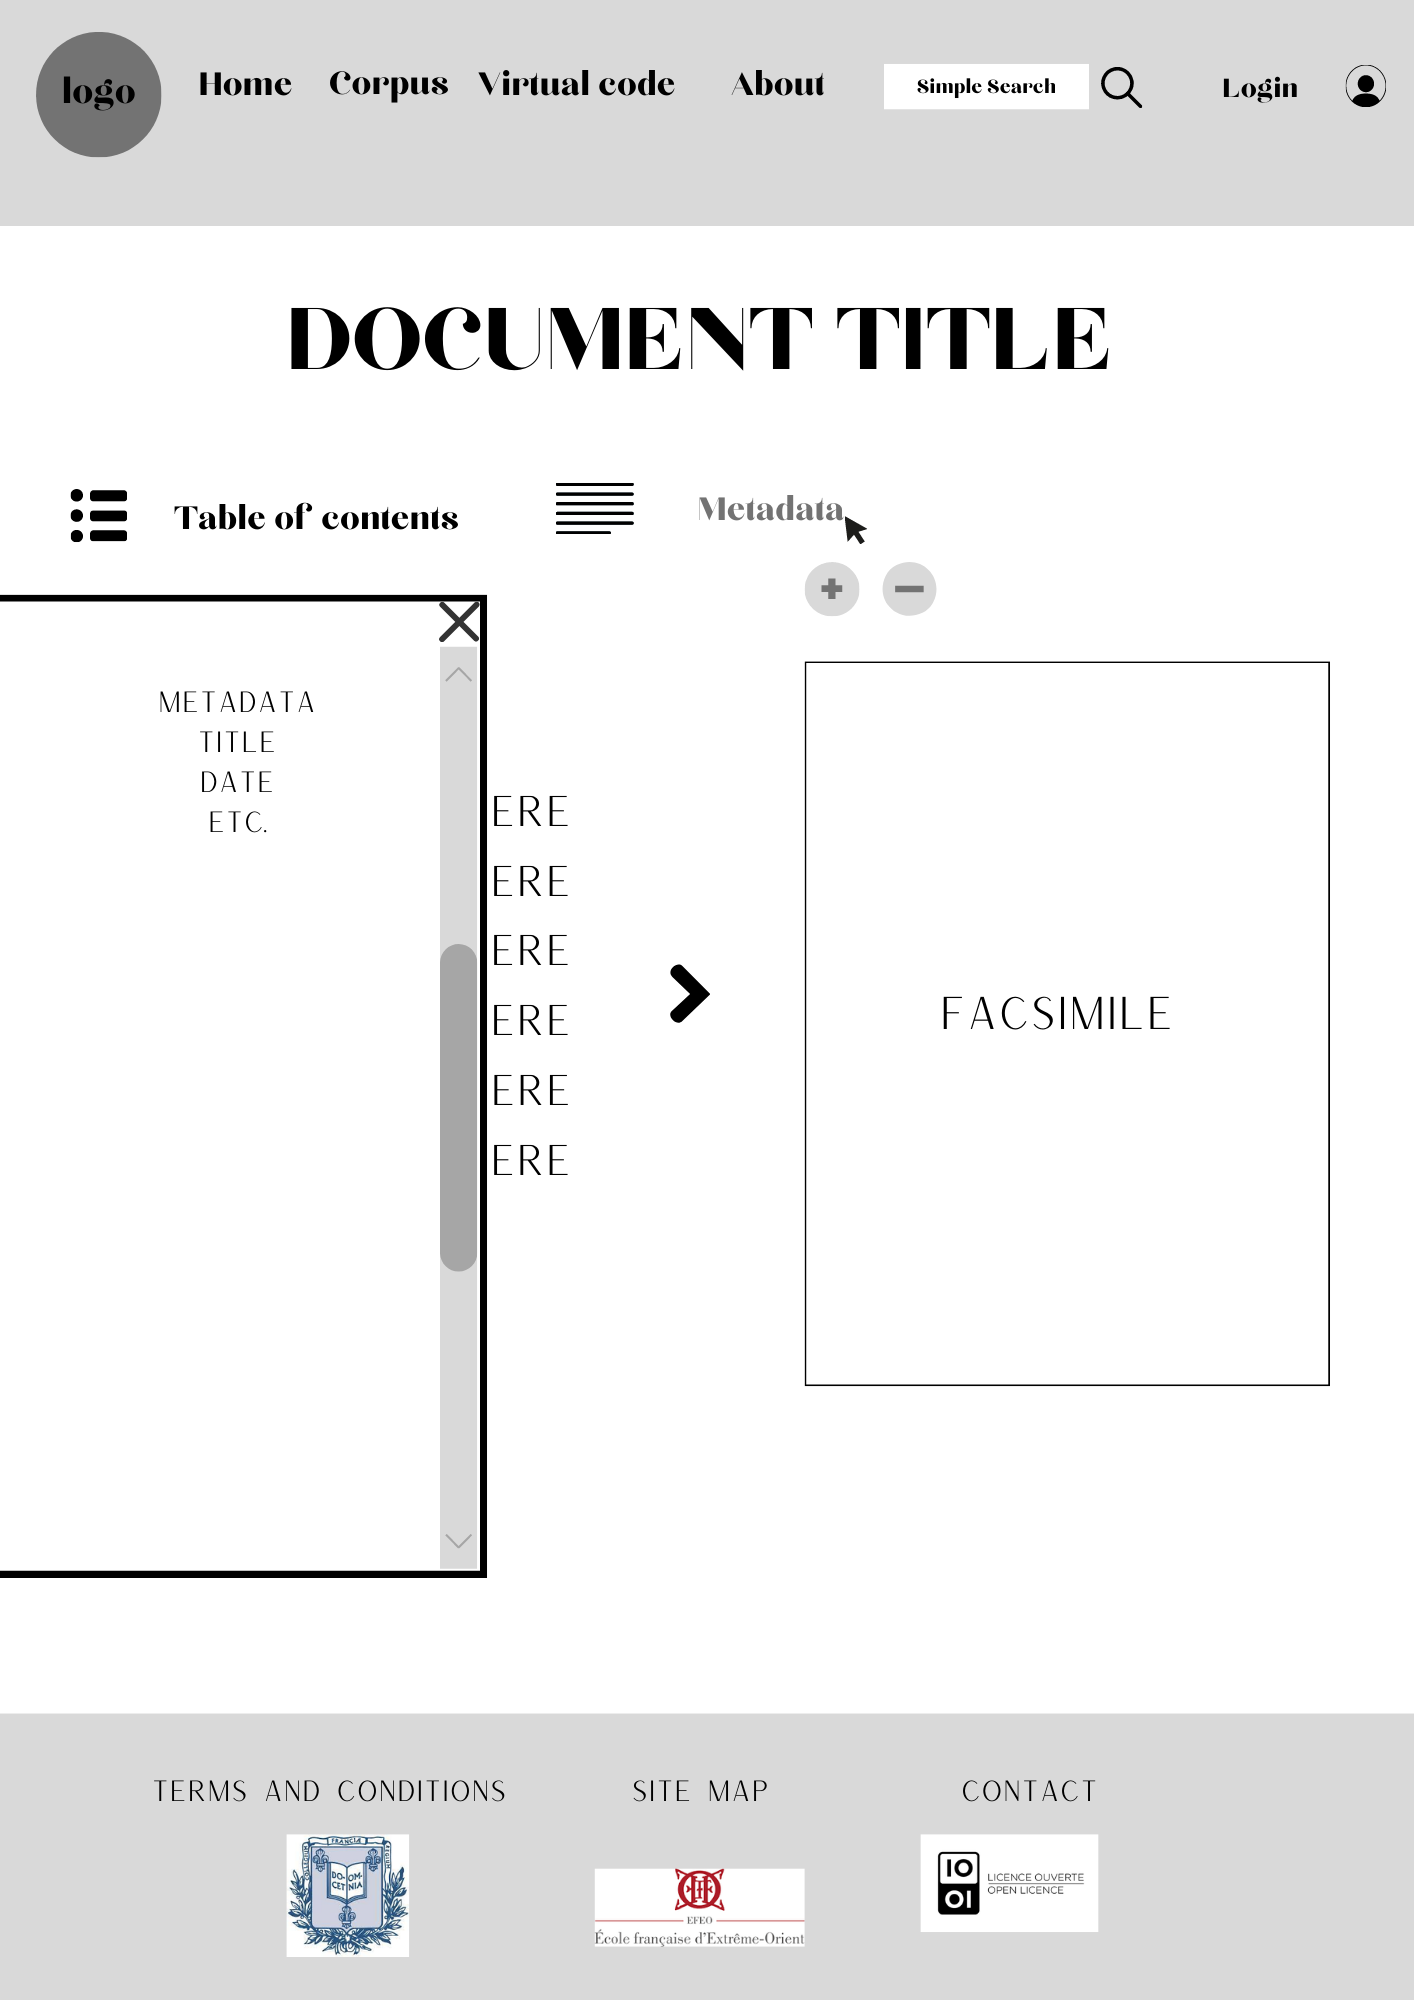
\includegraphics[width=\textwidth]{annexes/10 - Onglet métadonnées.png}
\noindent 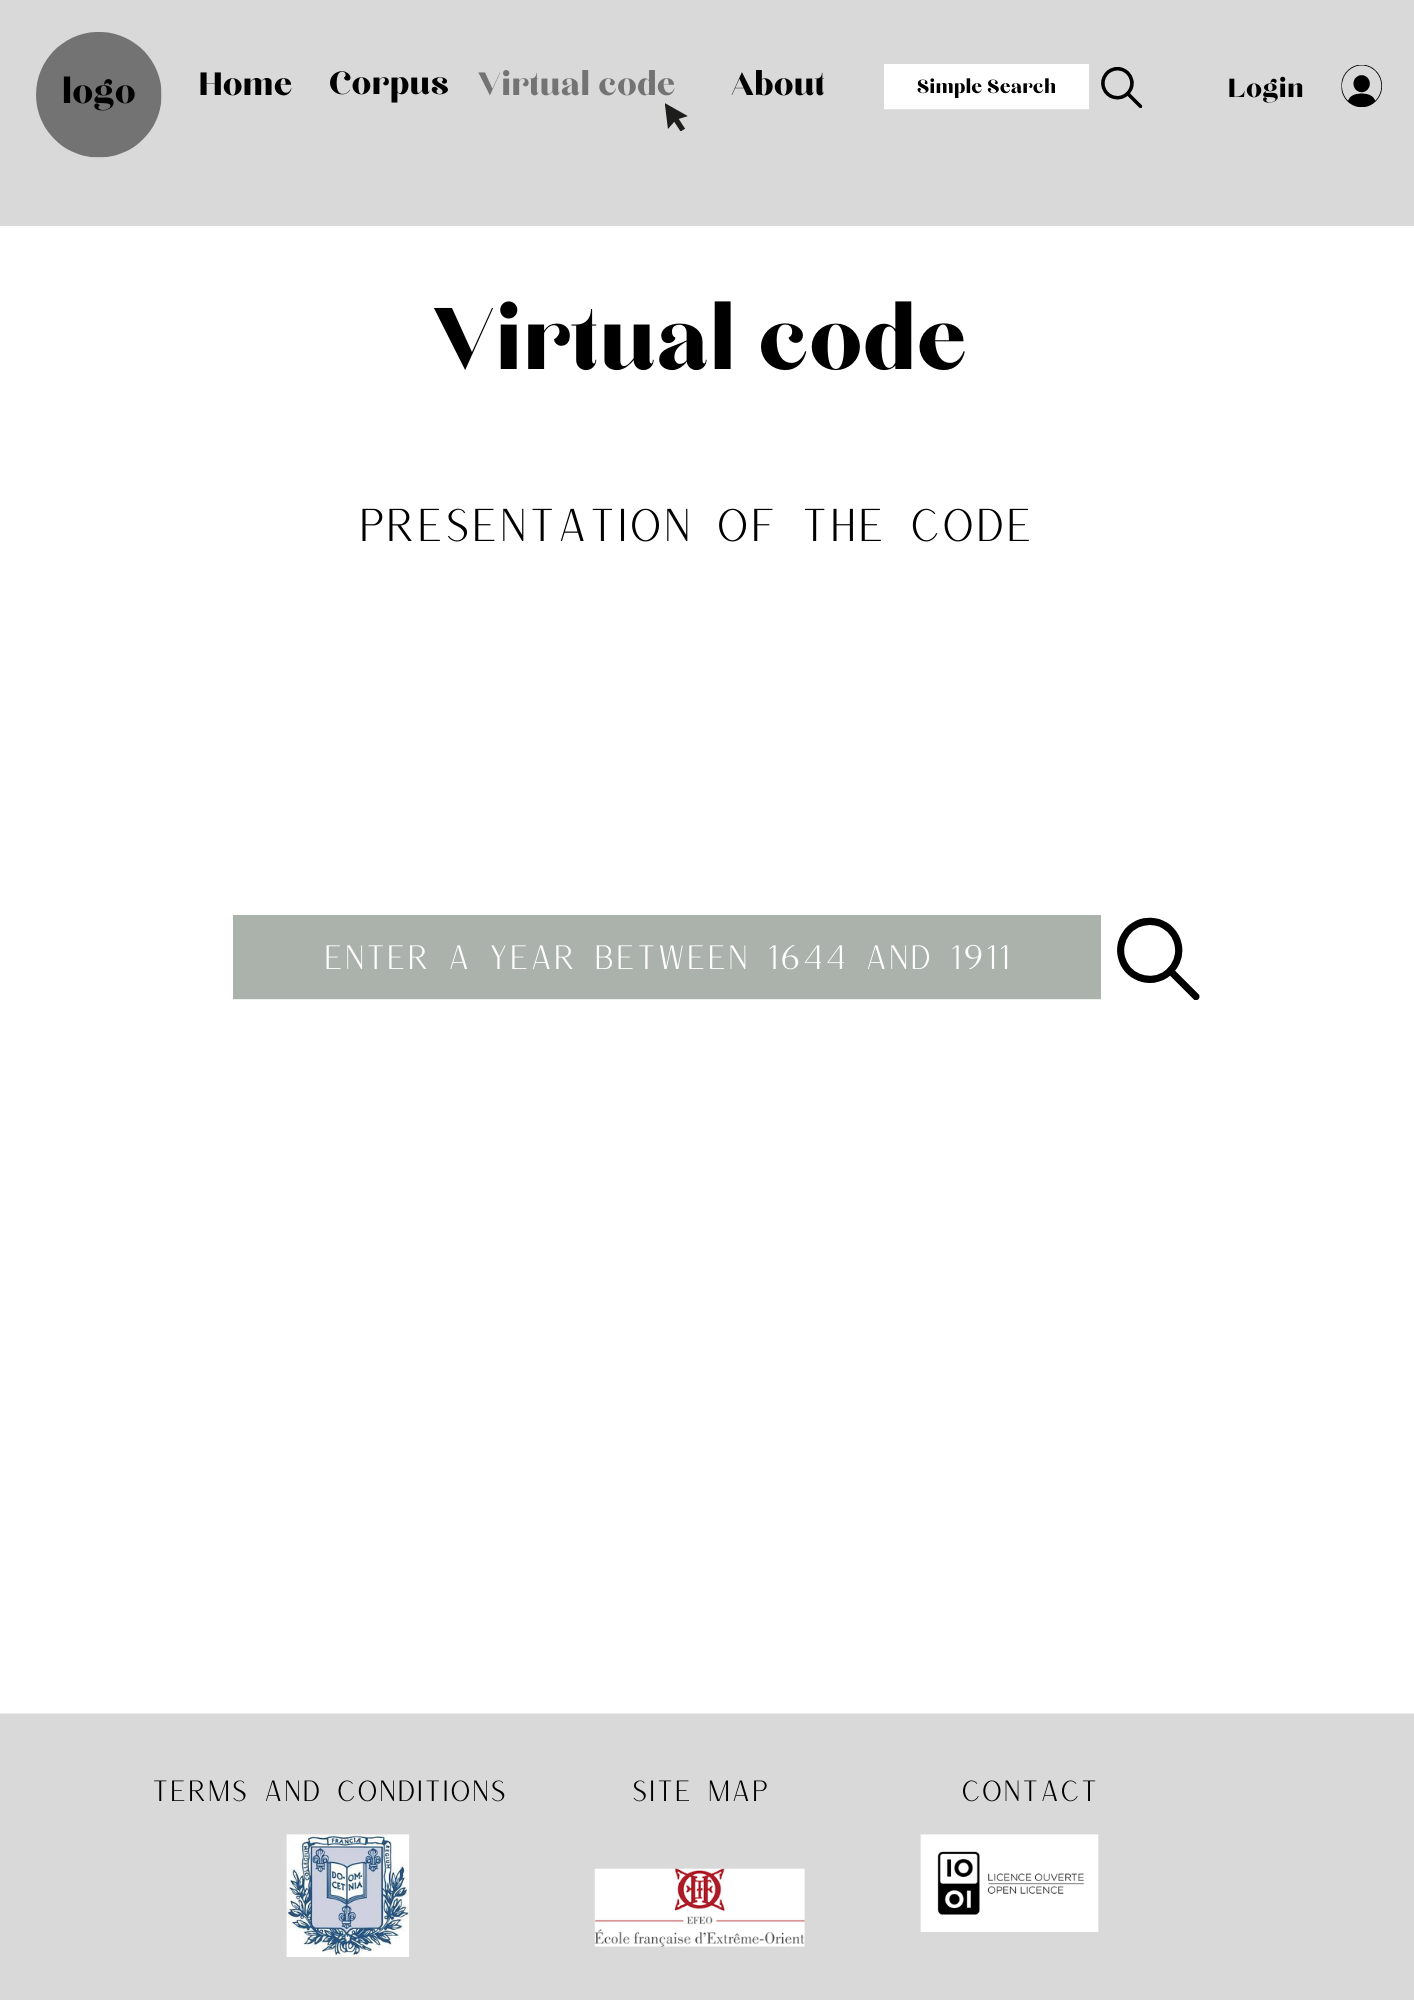
\includegraphics[width=\textwidth]{annexes/11 - Code virtuel (input).png}
\noindent 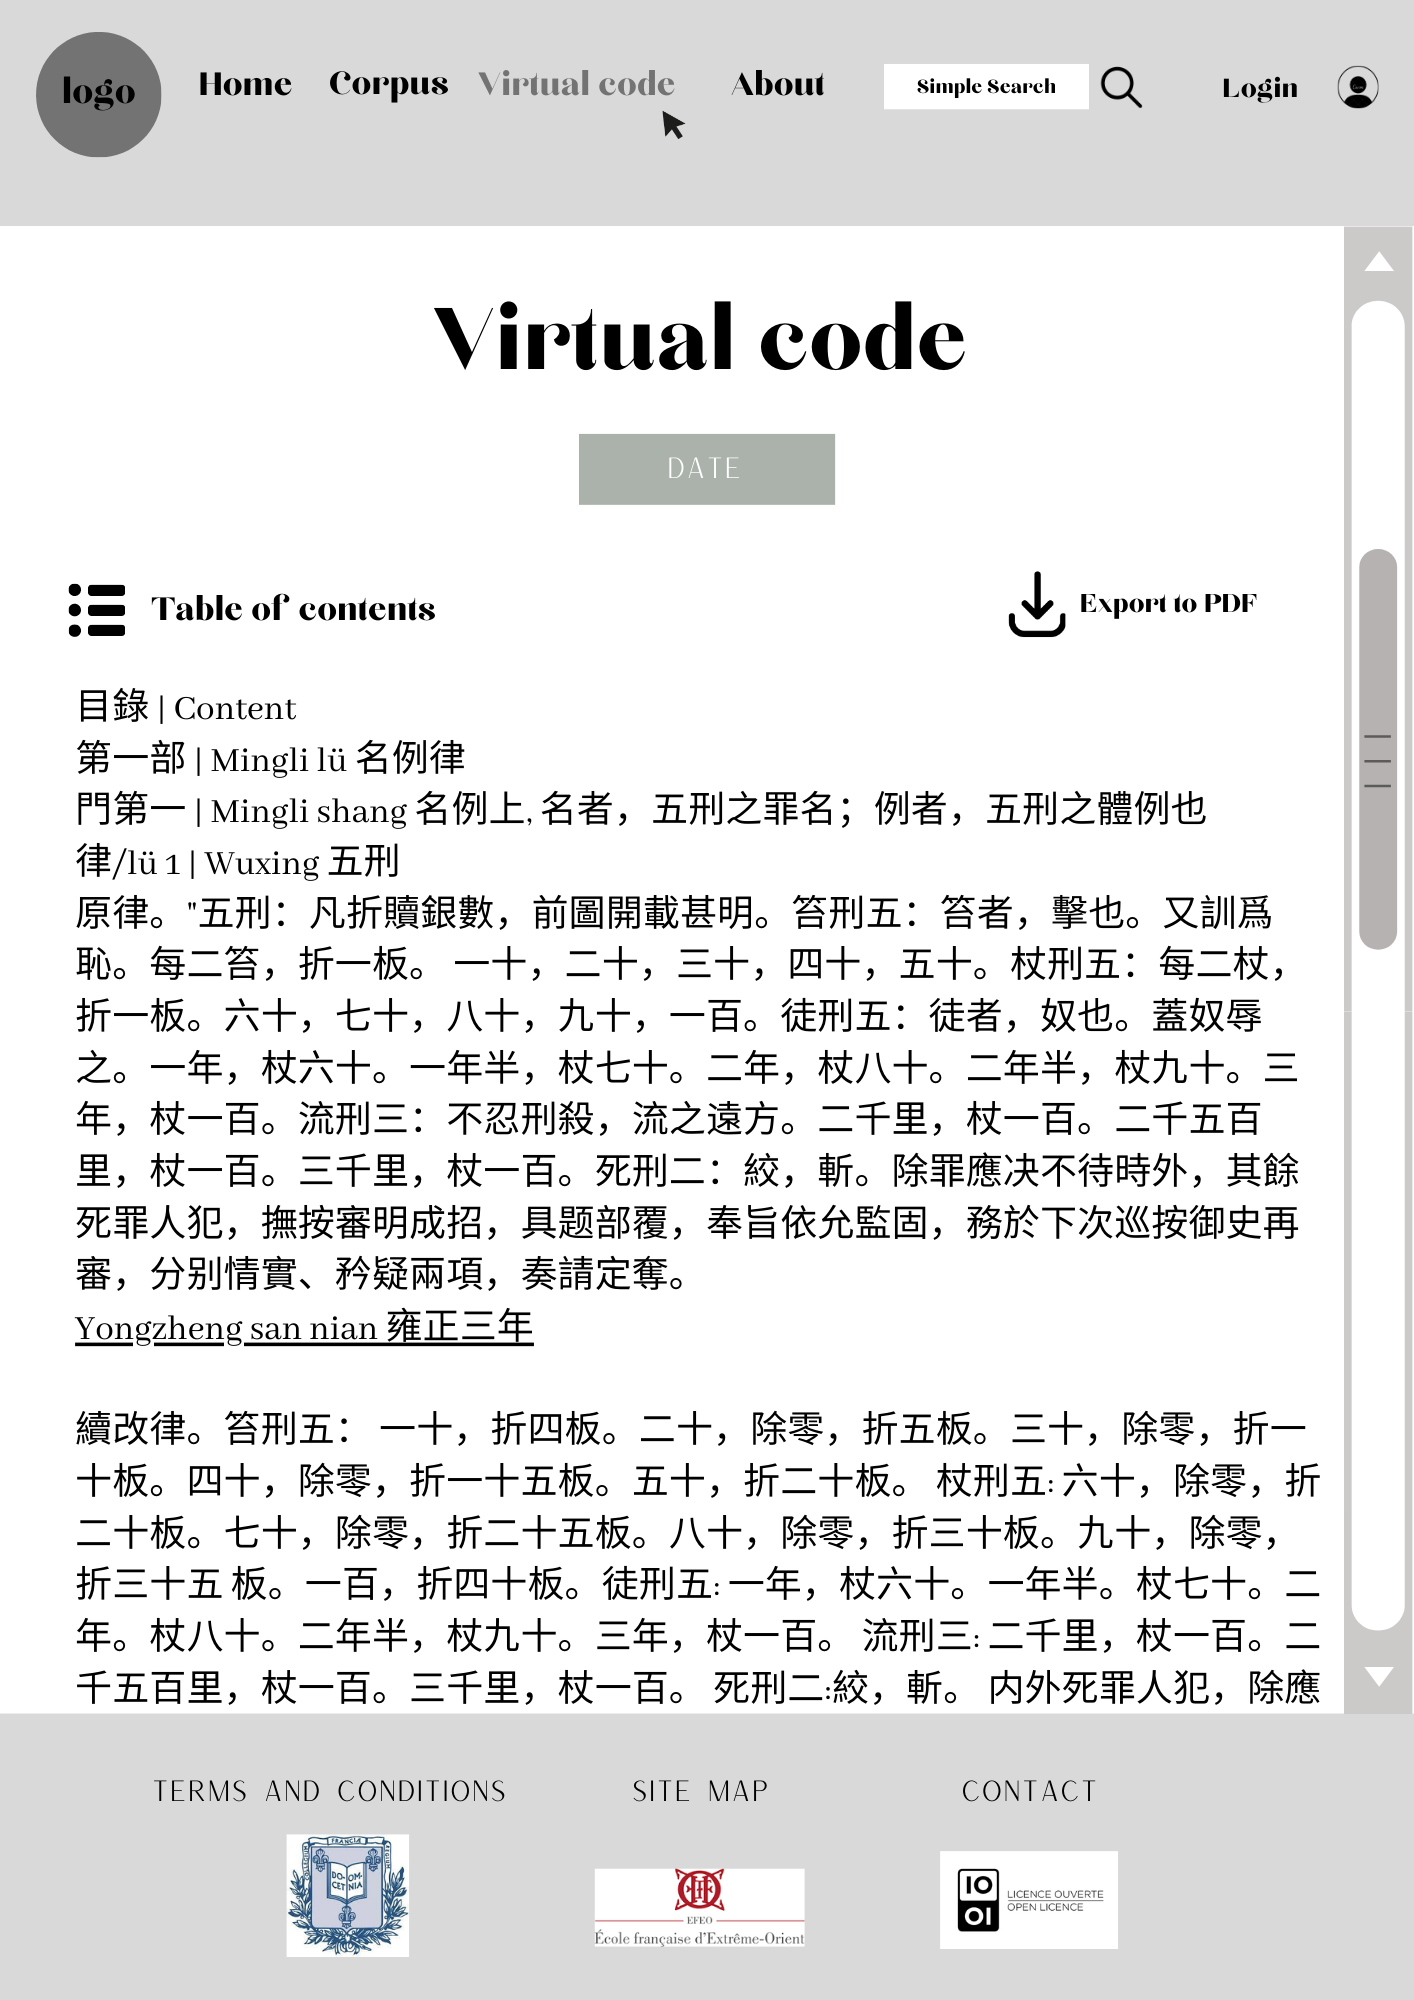
\includegraphics[width=\textwidth]{annexes/12 -Code virtuel (output).png}
\noindent 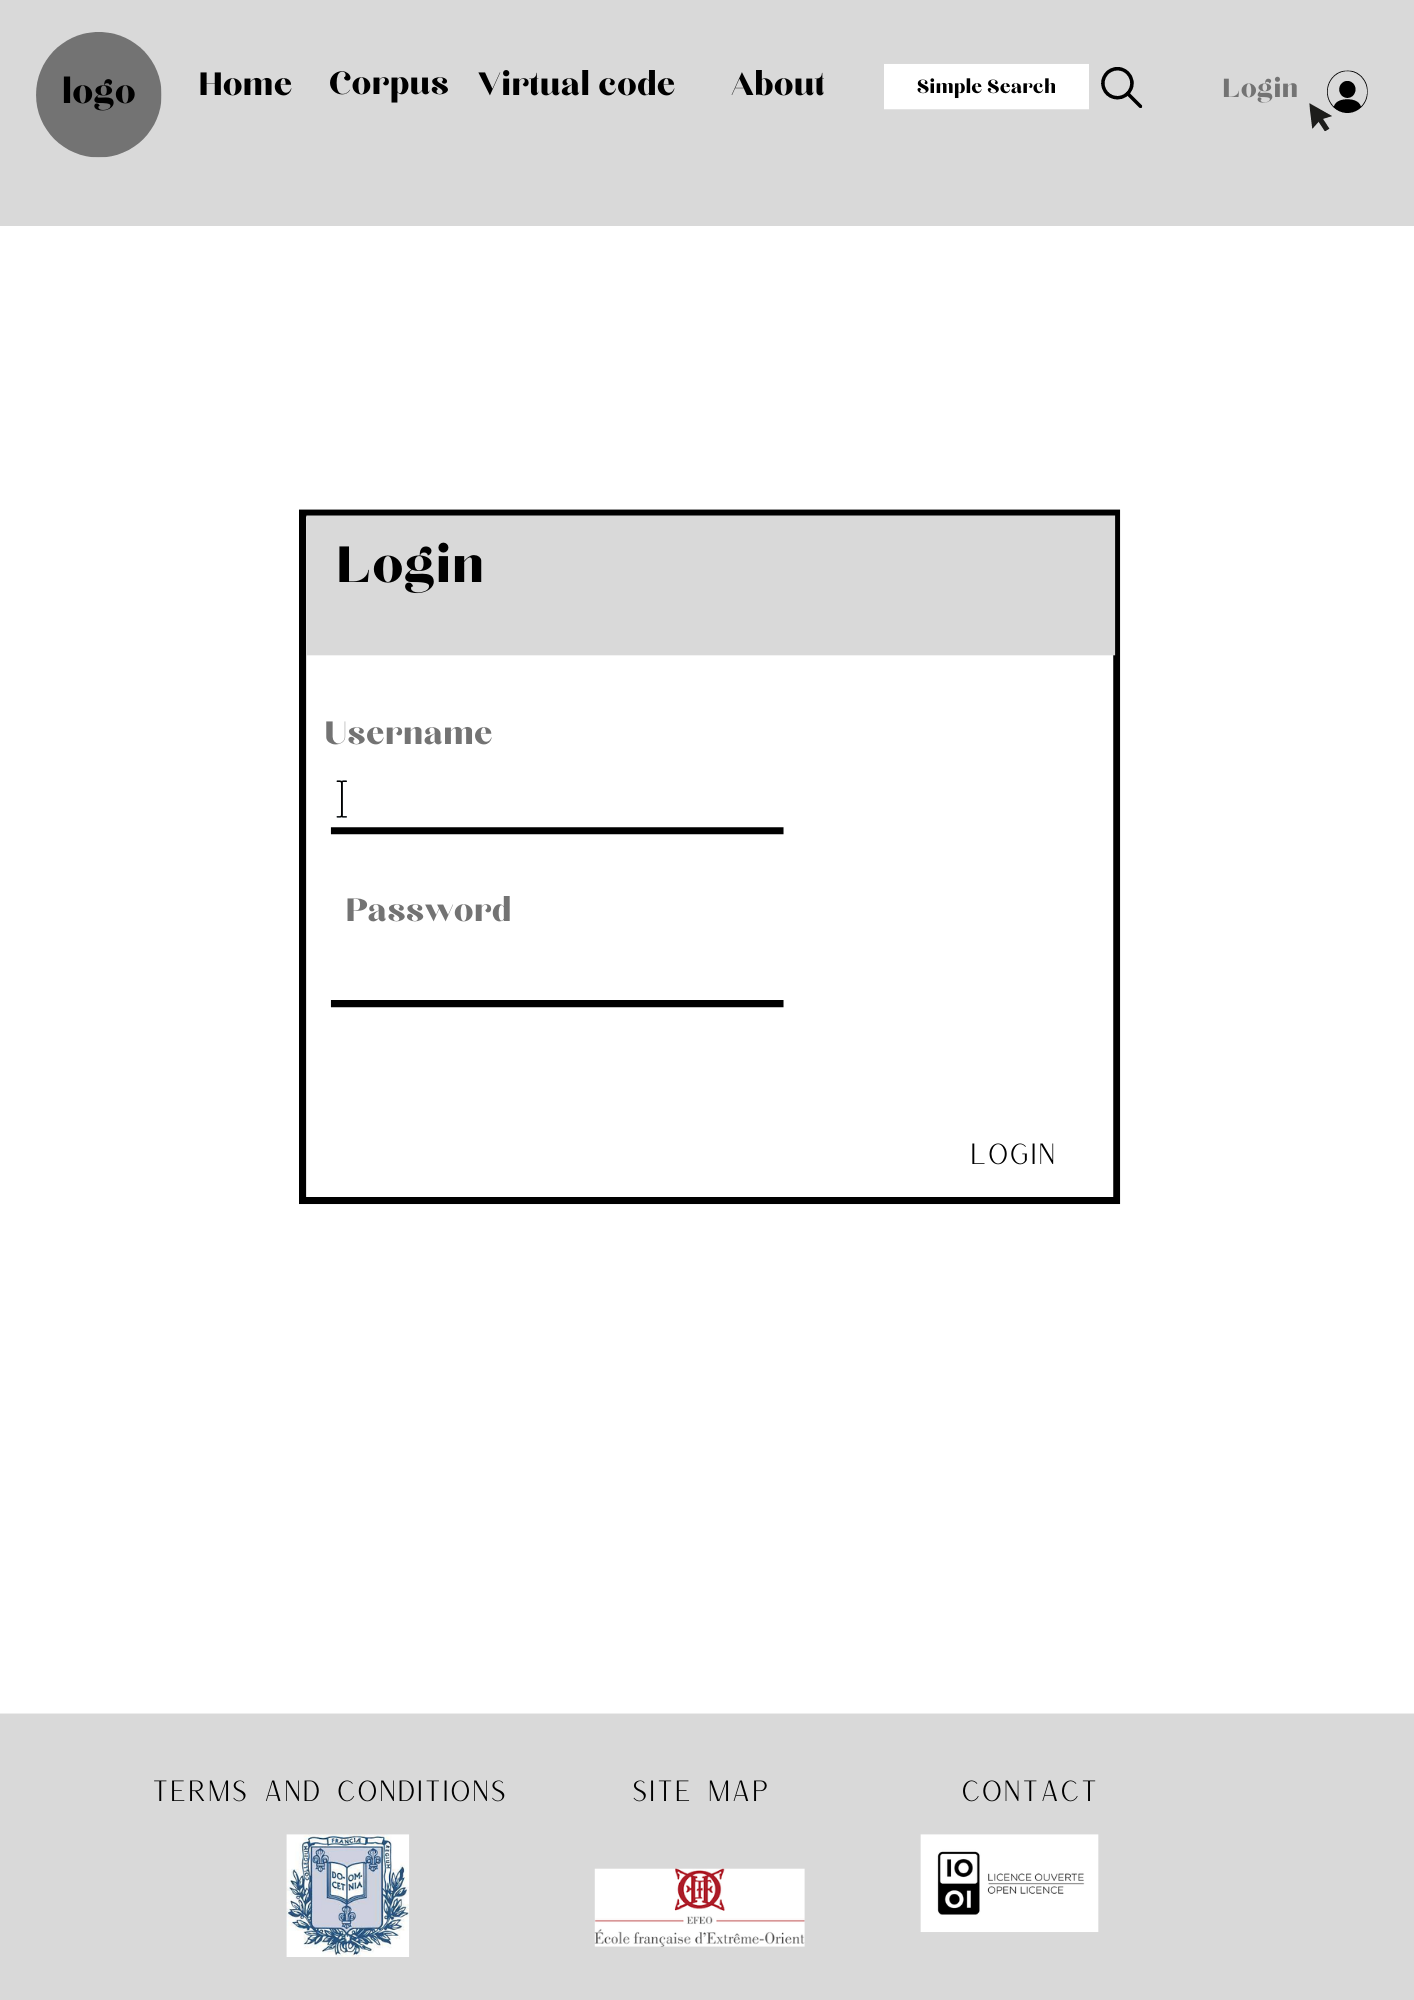
\includegraphics[width=\textwidth]{annexes/13 - Se connecter.png}
\noindent 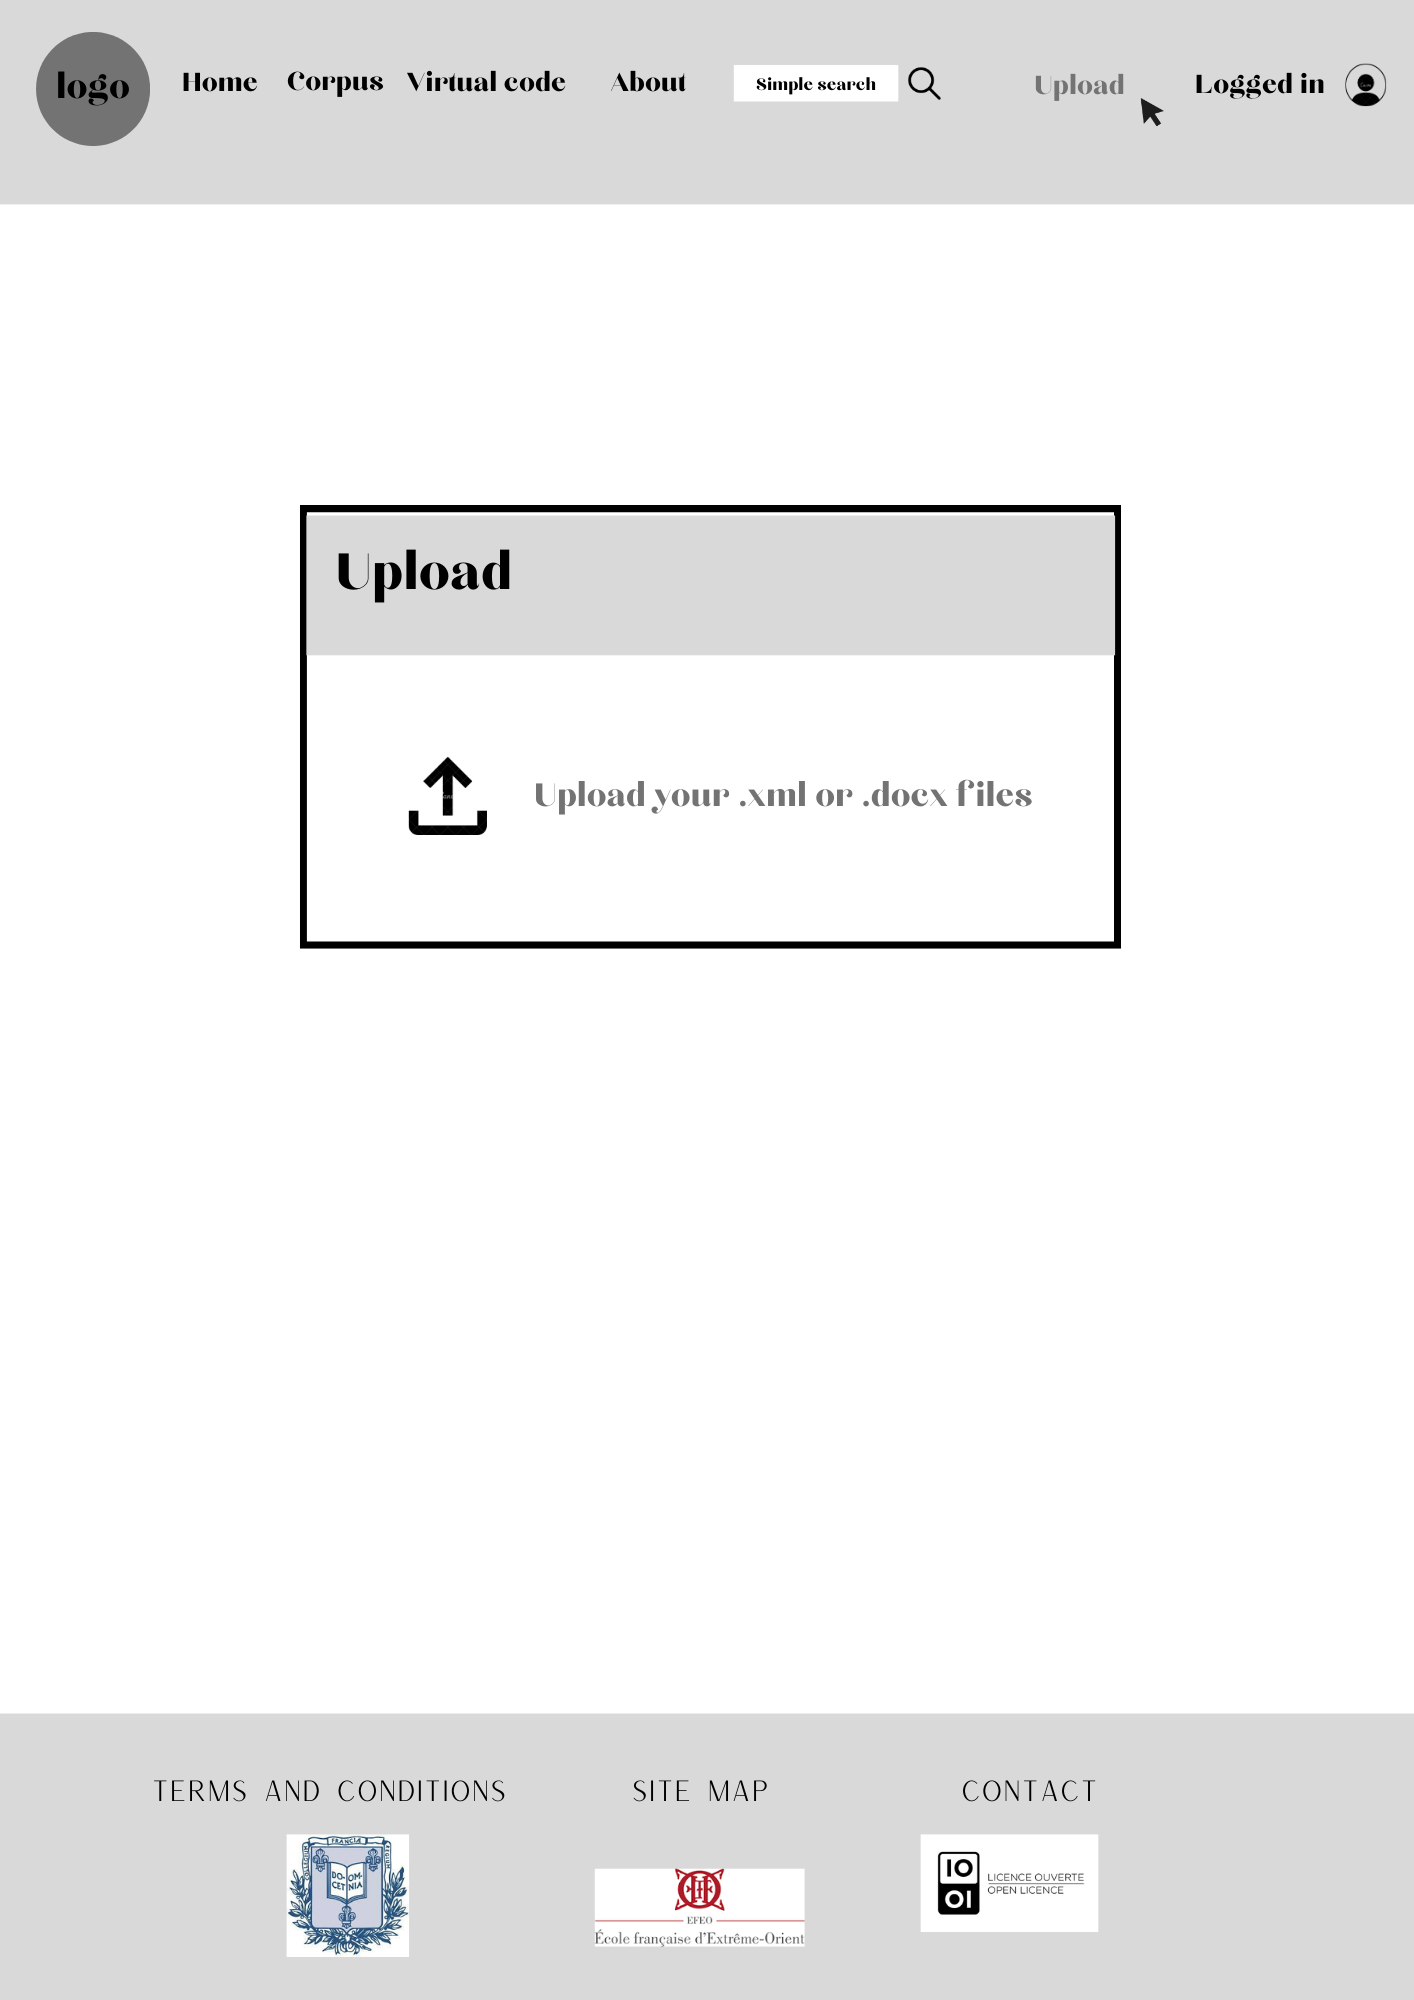
\includegraphics[width=\textwidth]{annexes/14 - Télécharger de nouveaux documents.png}

\section*{Liens}
\begin{itemize}
    \item 
\href{https://sharedocs.huma-num.fr/wl/?id=yHHcUPKWyusazIZqWVLgtbZI7J65OaLA&path=TEI%282%29&mode=grid}{Jeu de données \TEI de référence}
\item 
\href{}{Échantillon des données}
\item 
\href{https://sharedocs.huma-num.fr/wl/?id=yHHcUPKWyusazIZqWVLgtbZI7J65OaLA&path=ODD&mode=grid}{\ODD}
\item 
\href{}{\ODD pour l'affichage \tp}
\end{itemize}
\section*{Exemple d'affichage possible avec \tp}
\noindent 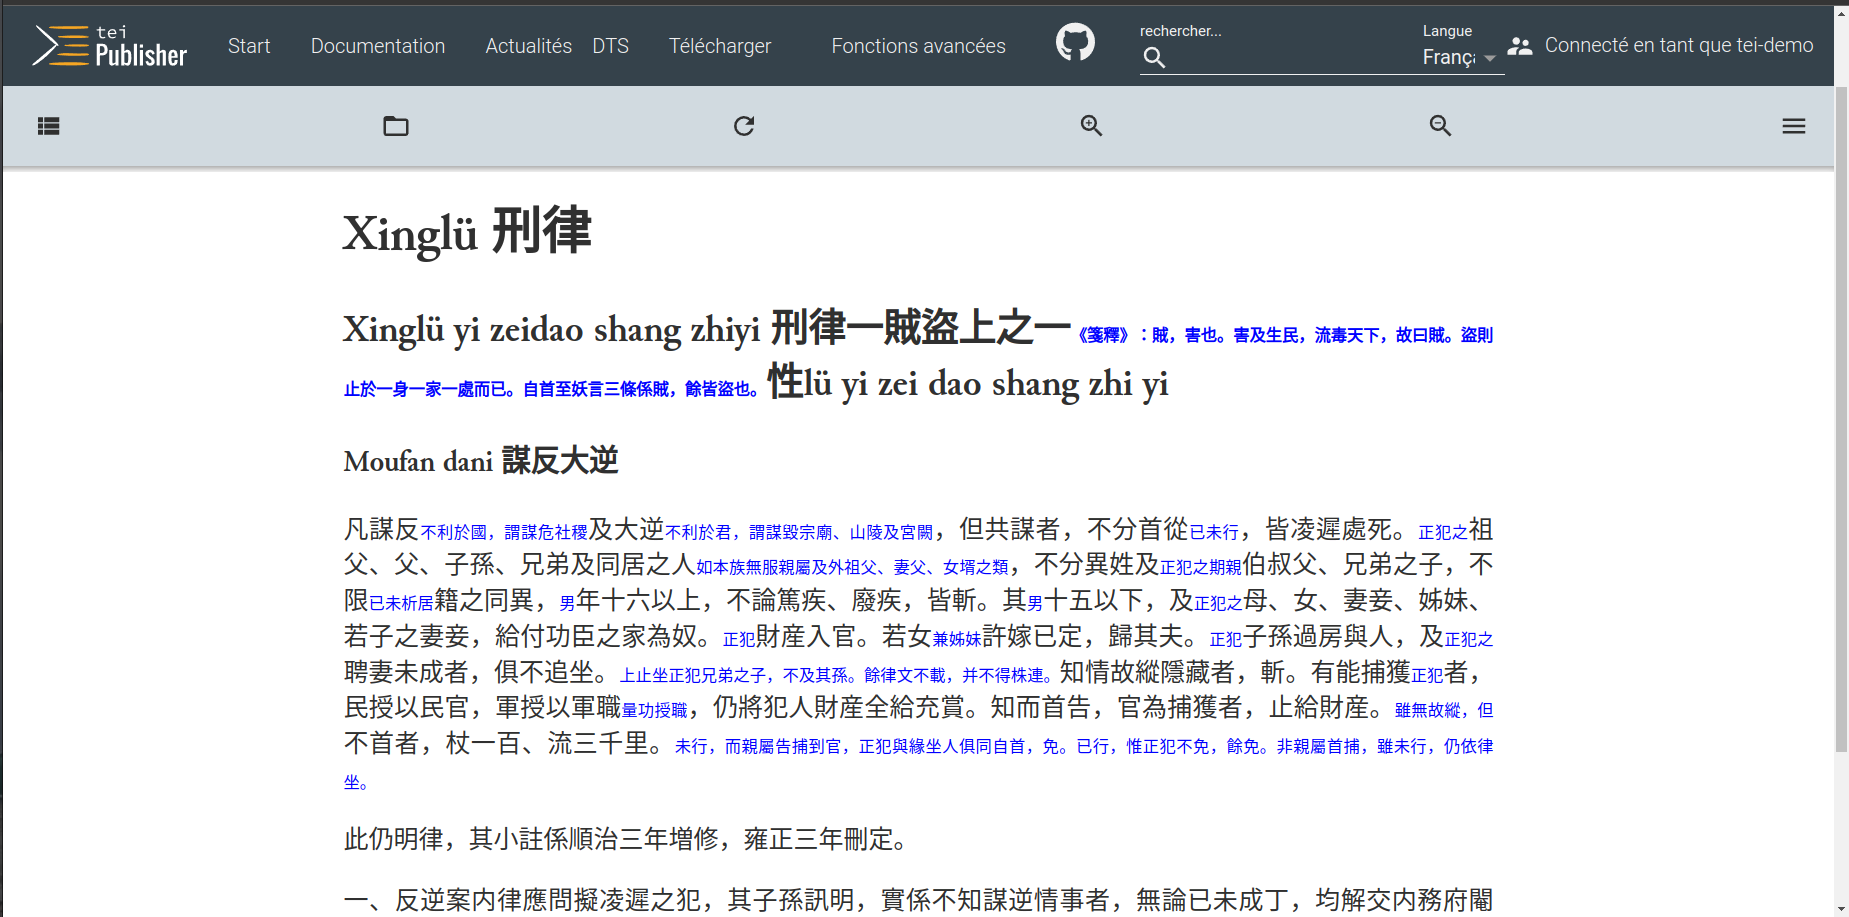
\includegraphics[width=\textwidth]{annexes/affichage.png}